% !TEX program = xelatex
\documentclass[a4paper]{article}
\usepackage[UTF8]{ctex}
\setCJKmainfont{SimSun}[BoldFont=SimHei,ItalicFont=KaiTi]
\setCJKsansfont{SimHei}
\usepackage[top=3mm,bottom=3mm,left=3.6mm,right=3.6mm]{geometry}
\usepackage{amsmath,amssymb,bm}
\usepackage{multicol}
\usepackage{tikz}
\usetikzlibrary{arrows.meta,calc}
\usepackage[dvipsnames]{xcolor}
\usepackage{enumitem,array,tabularx}
\pagestyle{empty}
\setlength{\parindent}{0pt}
\setlength{\parskip}{0pt}
\setlength{\columnsep}{2.35mm}
\setlength{\columnseprule}{0.13pt}
\setlength{\tabcolsep}{1.1pt}
\setlength{\fboxsep}{0.7pt}
\renewcommand{\baselinestretch}{0.690}
\setlist{nosep,leftmargin=6.2pt,labelsep=1pt,itemsep=0pt,parsep=0pt,topsep=0pt}
\definecolor{h}{HTML}{0B3D91}
\definecolor{b}{HTML}{1565C0}
\definecolor{o}{HTML}{E65100}
\definecolor{r}{HTML}{B71C1C}
\definecolor{g}{HTML}{1B5E20}
\definecolor{bg}{HTML}{EEF3FF}
\definecolor{warnbg}{HTML}{FFF2E6}
\definecolor{grid}{HTML}{D7DEE8}
\newsavebox{\fitbox}
\newcommand{\fitmath}[2][\dimexpr\linewidth-5pt\relax]{\sbox{\fitbox}{$\displaystyle #2$}\ifdim\wd\fitbox>#1\resizebox{#1}{!}{$\displaystyle #2$}\else\usebox{\fitbox}\fi}
\newcommand{\F}[1]{\colorbox{bg}{\fitmath{#1}}}
\newcommand{\FB}[1]{\par\noindent\colorbox{bg}{\begin{minipage}{\dimexpr\linewidth-2\fboxsep\relax}\centering\fontsize{5.05}{5.30}\selectfont\ensuremath{\displaystyle #1}\end{minipage}}\par}
\newcommand{\W}[1]{\colorbox{warnbg}{\fitmath{#1}}}
\newcommand{\mt}[1]{\vspace{0.4pt}{\fontsize{6.25}{6.50}\selectfont\bfseries\color{white}\colorbox{h}{\strut\ #1\ }}\par\vspace{0.2pt}}
\newcommand{\s}[1]{{\fontsize{5.45}{5.70}\selectfont\bfseries\color{b}$\blacktriangleright$ #1}\par}
\newcommand{\tagg}[1]{{\bfseries\color{o}#1}}
\newcommand{\bad}[1]{{\bfseries\color{r}#1}}
\newcommand{\ok}[1]{{\bfseries\color{g}#1}}
\newcommand{\slot}[2]{\textbf{#1}：#2\par}
\newcommand{\card}[2]{\vspace{0.25pt}\noindent\fcolorbox{grid}{white}{\begin{minipage}{0.972\linewidth}\textbf{\color{h}#1}\par #2\end{minipage}}\par\vspace{0.25pt}}
\newcommand{\chain}[1]{\par\noindent\colorbox{bg}{\begin{minipage}{\dimexpr\linewidth-2\fboxsep\relax}\fontsize{5.05}{5.30}\selectfont #1\end{minipage}}\par}
\newcommand{\warnline}[1]{\par\noindent\colorbox{warnbg}{\begin{minipage}{\dimexpr\linewidth-2\fboxsep\relax}\fontsize{5.05}{5.30}\selectfont\bad{反制}：#1\end{minipage}}\par}
\newcommand{\tinyflow}[1]{\begin{center}\vspace{-2pt}#1\vspace{-4pt}\end{center}}
\newcommand{\pipefig}{\tinyflow{\begin{tikzpicture}[>=Latex,scale=.50,every node/.style={font=\tiny}]
\draw[blue] (0,1.2)--(.7,1.2);\draw[thick](0,1.2)--(0,0)--(.8,0)..controls(1.1,0)and(1.1,.45)..(1.55,.45)--(3.2,.45);\draw[thick](.2,1.2)--(.2,.2)--(.82,.2)..controls(1.0,.2)and(1.1,.65)..(1.55,.65)--(3.2,.65);\node[circle,draw,inner sep=1pt] at (2.0,.55){P};\draw[->,blue](-.1,.1)--(.55,.1);\draw[->,blue](2.35,.55)--(3.0,.55);\draw[<->](1.95,.55)--(1.95,-.25);\node[right]at(1.95,.1){$h$};\node at(.1,1.45){水面1};\node at(2.9,.9){2出口/泵后};\end{tikzpicture}}}
\newcommand{\hydrofig}{\tinyflow{\begin{tikzpicture}[>=Latex,scale=.50,every node/.style={font=\tiny}]
\draw[thick](0,1.4)--(0,0)--(1.0,0)--(1.0,1.4);\draw[blue](.05,1.0)--(.95,1.0);\node at(.5,1.25){U管};\draw[thick](1.7,0)--(3.1,.25)--(3.1,1.3)--(1.7,1.05)--cycle;\draw[->,red](1.45,.55)--(2.2,.55);\draw[->,red](1.7,.25)--(2.6,.95);\node at(2.45,1.55){闸门/曲面};\end{tikzpicture}}}
\newcommand{\cvfig}{\tinyflow{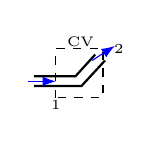
\begin{tikzpicture}[>=Latex,scale=.50,every node/.style={font=\tiny}]
\draw[thick](0,.3)--(1.2,.3)--(1.8,.95);\draw[thick](0,.55)--(1.05,.55)--(1.55,1.1);\draw[dashed](.55,.0)rectangle(1.75,1.25);\draw[->,blue](-.15,.42)--(.55,.42);\draw[->,blue](1.47,.95)--(2.05,1.32);\node at(.55,-.18){1};\node at(2.15,1.25){2};\node at(1.18,1.43){CV};\end{tikzpicture}}}
\newcommand{\potfig}{\tinyflow{\begin{tikzpicture}[>=Latex,scale=.48,every node/.style={font=\tiny}]
\foreach \y in{-.45,0,.45}{\draw[->,blue](-.2,\y)--(.9,\y);}\draw[thick](1.3,0)circle(.38);\node at(1.3,-.65){圆柱};\draw[fill=black](2.35,0)circle(.04);\node[above]at(2.35,0){源};\draw[fill=black](3.35,0)circle(.04);\node[above]at(3.35,0){汇};\draw[thick](2.75,-.55)..controls(3.1,-.8)and(3.55,-.8)..(3.9,-.55);\draw[thick](2.75,.55)..controls(3.1,.8)and(3.55,.8)..(3.9,.55);\draw[thick](4.5,-.65)--(4.5,.75);\draw[fill=black](5.0,.25)circle(.04);\draw[fill=black](4.0,.25)circle(.04);\node at(4.5,-.9){镜像壁};\end{tikzpicture}}}
\newcommand{\lavalfig}{\tinyflow{\begin{tikzpicture}[>=Latex,scale=.48,every node/.style={font=\tiny}]
\draw[thick](0,.7)..controls(.8,.55)and(1.0,.23)..(1.65,.23)..controls(2.3,.23)and(2.55,.65)..(3.5,.8);\draw[thick](0,-.7)..controls(.8,-.55)and(1.0,-.23)..(1.65,-.23)..controls(2.3,-.23)and(2.55,-.65)..(3.5,-.8);\draw[dashed](1.65,-.55)--(1.65,.55);\node at(1.65,-.75){喉$A^*$};\draw[->,blue](-.25,0)--(.55,0);\draw[->,blue](2.75,0)--(3.6,0);\node at(.35,1.02){$p_0,T_0$};\node at(3.25,1.05){$p_e,p_b$};\draw[red,thick](2.45,-.55)--(2.45,.55);\node[red]at(2.75,.68){激波?};\end{tikzpicture}}}
\newcommand{\shockfig}{\tinyflow{\begin{tikzpicture}[>=Latex,scale=.48,every node/.style={font=\tiny}]
\draw[->,blue](-.1,.42)--(.85,.42);\node at(.45,.68){$M_1$};\draw[thick](.85,0)--(2.25,0);\draw[thick](.85,0)--(2.25,.48);\draw[red,thick](.85,0)--(1.55,1.0);\node[red]at(1.28,1.02){$\beta$};\node at(2.05,.72){$\theta$};\draw[->,blue](1.75,.35)--(2.5,.6);\draw[thick](3.0,0)--(4.35,0);\draw[thick](3.0,0)--(4.35,-.48);\foreach \a in{0,.15,.3,.45}{\draw[red](3.0,0)--(3.85,-\a);}\node at(3.85,-.82){PM扇};\end{tikzpicture}}}
\newcommand{\visfig}{\tinyflow{\begin{tikzpicture}[>=Latex,scale=.48,every node/.style={font=\tiny}]
\draw[thick](0,0)--(2.0,0);\draw[thick](0,.7)--(2.0,.7);\draw[->,red](.4,.7)--(1.4,.7);\node at(1.55,.9){$U$};\draw[blue,thick](.05,0)..controls(.85,.25)and(1.4,.55)..(1.95,.7);\node at(1,-.23){Couette/Poiseuille};\draw[thick](2.7,0)circle(.5);\draw[blue,thick](2.7,0)..controls(3.0,.25)and(3.0,.45)..(3.0,.7);\node at(2.7,-.75){圆管剖面};\end{tikzpicture}}}
\newcommand{\blfig}{\tinyflow{\begin{tikzpicture}[>=Latex,scale=.48,every node/.style={font=\tiny}]
\draw[thick](0,0)--(2.7,0);\draw[->,blue](-.2,.55)--(.75,.55);\node at(.25,.82){$U$};\draw[red,thick](0,0)..controls(.8,.2)and(1.7,.48)..(2.7,.75);\draw[dashed](2.1,0)--(2.1,.60);\node[right]at(2.1,.3){$\delta$};\draw[thick](3.55,0)circle(.55);\draw[red,thick](3.05,.15)..controls(3.55,.55)and(4.05,.55)..(4.35,.1);\node at(3.55,-.75){外绕物};\end{tikzpicture}}}
\newcommand{\kinfig}{\tinyflow{\begin{tikzpicture}[>=Latex,scale=.48,every node/.style={font=\tiny}]
\draw[->](0,0)--(1.6,0)node[right]{$x$};\draw[->](0,0)--(0,1.1)node[above]{$y$};\draw[blue,->](.25,.2)..controls(.7,.55)and(1.0,.62)..(1.45,.9);\node at(.9,.2){流线};\draw[thick](2.2,0)--(3.2,.75);\draw[->,red](2.7,.38)--(2.45,.72);\node at(2.85,.85){$\bm n$};\node at(2.85,.15){面};\end{tikzpicture}}}
\begin{document}
\fontsize{5.25}{5.45}\selectfont

% ================= PAGE 1 =================
\begin{multicols}{2}
\mt{母题迁移总图：高难母题 $\to$ 模板 $\to$ 弱化题}
\card{考场用法}{不按章节翻。先看\tagg{图形/装置/边界条件}，把题归入母题；再套固定变量和公式链。弱化题通常只是母题少给一个部件、少求一个量、或只问判断。}
\s{统一变量命名}
截面统一为 $1,2,3$；控制体用 CV；入口/出口按质量流向定；$x$ 水平、$y$ 向上；外法向 $\bm n$ 指出控制体；压力默认用\tagg{表压}，气体/可压题常用\tagg{绝压}。\par
\F{Q=AV,\quad \dot m=\rho Q,\quad Re=VL/\nu=\rho VL/\mu}\quad \F{Ma=V/a,\ a=\sqrt{\gamma RT}}
\s{所有计算题的第一行}
\chain{1 判模型：静水 / 能量 / CV动量 / 势流 / 可压 / 粘性 / 边界层 / 相似。\quad 2 写适用条件。\quad 3 画截面和方向。\quad 4 按公式链推进。\quad 5 检查单位、正负、表压绝压、查表入口。}
\s{母题索引}
\begin{tabularx}{\linewidth}{|p{.29\linewidth}|X|}\hline
管路泵损失 & 水池-管-泵-阀-弯头-压力表；求$Q,H,P,h$。\\\hline
静水闸门 & 静止液体、U管、倾斜/曲面闸门、浮体。\\\hline
CV动量 & 弯管、喷流打板、叶片、射流反力。\\\hline
势流叠加 & 源汇涡偶极、圆柱、镜像、环量、升力。\\\hline
Laval可压 & 大容器-喷管-背压、阻塞、出口/管内激波。\\\hline
激波/膨胀 & 楔面、斜激波、PM膨胀扇、超声速转角。\\\hline
粘性剪切 & 两板、圆管层流、两层流体、N-S简化。\\\hline
边界层阻力 & 平板/圆柱/球外绕，求$\delta,C_f,D$。\\\hline
运动/应力/相似 & 速度场、应力张量、$\pi$定理、模型试验。\\\hline
\end{tabularx}
\s{变量和方向反制}
压力力永远作用在\tagg{受压面法向}；CV动量右边永远是\tagg{流出动量-流入动量}；题问“管对流体”与“流体对管”相反；绝压=表压+$p_a$；能量方程用水头时每项单位是 m，用压强式每项 Pa。

\mt{母题1：水池-管路-泵-阀-弯头综合题}
\pipefig
\slot{图形特征}{水面/水箱 + 管道 + 泵/水轮机 + 弯头阀门 + 压力表或汽蚀高度。}
\slot{关键词}{流量、扬程、输出功率、局部阻力、沿程损失、粗糙度、Moody、进口压力、汽化压力。}
\slot{变量}{1=上游水面或入口，2=泵前，3=泵后/出口；$z$ 向上；$V_i=Q/A_i$。}
\slot{顺序}{先由 $Q$ 或未知 $Q$ 设 $V$；算 $Re$；取 $\lambda$；汇总损失；列机械能；最后算 $P$ 或 $h$。}
\chain{公式链：$V_i=Q/A_i\to Re_i=V_id_i/\nu\to \lambda_i$；层流$64/Re$，湍流查Moody\par
$h_f=\sum \lambda_i(L_i/d_i)V_i^2/(2g)$，$h_\zeta=\sum \zeta_j V_j^2/(2g)$\par
$z_1+p_1/\rho g+\alpha_1V_1^2/2g+H_p-H_t=z_3+p_3/\rho g+\alpha_3V_3^2/2g+h_f+h_\zeta$\par
$P_{pump}=\rho gQH_p/\eta$，$P_T=\eta\rho gQH_t$}
\slot{变体迁移}{多一个弯头：只加 $\zeta V^2/2g$；换管径：分段算$V_i$；斜管：只改$z$；求粗糙度：由能量反推$\lambda$再查Moody；吸水泵高度：用泵前截面压力约束 $p_2\ge p_v+\Delta p_{safe}$。}
\warnline{局部损失用\tagg{所在管段速度头}，不是统一速度；水面 $V\approx0$；压力表读数是表压；泵加能写左边，水轮机取能写右边或负泵头。}

\mt{母题2：静水压力-测压管-闸门/曲面}
\hydrofig
\slot{图形特征}{液体静止；U形管/差压计；平面闸门、倾斜门、圆弧门、浸没物体。}
\slot{关键词}{静水压强、压力中心、合力、铰链力、浮力、测压管、表压、真空。}
\slot{变量}{自由面为0基准；受压面形心$c$；压力中心$p$；深度$h$向下为正。}
\slot{顺序}{先统一压强基准；求形心压强；求合力；定位压力中心；再对铰链取矩或分解曲面力。}
\chain{公式链：$p=p_0+\rho gh$；表压用$p_g=\rho gh$\par
平面：$F=p_cA=\rho gh_cA$，$h_p=h_c+I_G/(h_cA)$\par
倾斜面沿板：$s_p=s_c+I_G/(s_cA)$，$h=s\sin\theta$\par
曲面：$F_H=$投影面静水压力；$F_V=$曲面上方液体重；$R=\sqrt{F_H^2+F_V^2}$\par
浮力：$F_B=\rho gV_{disp}$}
\slot{变体迁移}{上方有气压：全体加$p_0A$；液体换密度：分层积分；闸门倾斜：深度仍是竖直深度；曲面门：水平/竖直分量分开。}
\warnline{压力中心比形心\tagg{更深}；不要把斜长当竖直深度；U管两端同高同液连通处压强相等；绝压不能为负，表压可以为负。}

\mt{母题3：CV动量-弯管-喷流-叶片受力}
\cvfig
\slot{图形特征}{流体转弯、喷流撞板/叶片、管道支座反力、速度方向改变。}
\slot{关键词}{作用力、支承力、喷射反力、动量方程、控制体、速度分量、偏转角。}
\slot{变量}{CV 包住流体；1入口、2出口；$x/y$固定；$\bm R$为外界对CV的未知力。}
\slot{顺序}{先由连续/能量求$V,p$；再列$x/y$动量；解出外界对流体力；题要管受力则取反。}
\chain{公式链：$\dot m=\rho Q$，$V_x=V\cos\theta$，$V_y=V\sin\theta$\par
$\sum F_x=\dot m(V_{2x}-V_{1x})$，$\sum F_y=\dot m(V_{2y}-V_{1y})$\par
$F_p=pA$ 指向CV内部；重力 $G=\rho gV_{CV}$；自由射流$p=p_a$表压0\par
叶片功：$P=\rho Q(u_1V_{u1}-u_2V_{u2})$；力矩：$M=\dot m(r_2V_{u2}-r_1V_{u1})$}
\slot{变体迁移}{弯头多段：只关心入口/出口动量，内部弯曲进损失；喷流打板：出口压力表压0；运动叶片：速度三角形用相对速度；要求支座力：流体对管=管对流体反向。}
\warnline{动量方程方向最容易错；先写“外力对流体”，最后再反向；压力力只在截面上出现，表压出口到大气为0。}

\par\medskip

\mt{母题4：势流叠加-圆柱-镜像-环量升力}
\potfig
\slot{图形特征}{无限平面无粘不可压；源/汇/涡/偶极；壁面镜像；圆柱绕流；带环量。}
\slot{关键词}{势函数、流函数、无旋、不可压、驻点、流线、镜像法、圆柱表面压力、升力。}
\slot{变量}{$r,\theta$ 极坐标；来流 $U$ 沿$x$；圆柱半径$a$；环量$\Gamma$；壁面是$\psi=$常数。}
\slot{顺序}{先写基本流；线性叠加得到$\varphi/\psi$；由速度公式求驻点/边界；表面速度进Bernoulli；积分或定理求力。}
\chain{基本流：均匀流 $\varphi=Ur\cos\theta,\psi=Ur\sin\theta$\par
源/汇：$v_r=\pm Q/(2\pi r)$，$\varphi=\pm(Q/2\pi)\ln r$，$\psi=\pm(Q/2\pi)\theta$\par
涡：$v_\theta=\Gamma/(2\pi r)$，$\varphi=(\Gamma/2\pi)\theta$，$\psi=-(\Gamma/2\pi)\ln r$\par
偶极：$\varphi=M\cos\theta/r$，$\psi=-M\sin\theta/r$\par
圆柱：$\varphi=U(r+a^2/r)\cos\theta$；$v_r=U(1-a^2/r^2)\cos\theta$；$v_\theta=-U(1+a^2/r^2)\sin\theta+\Gamma/(2\pi r)$\par
表面：$v_\theta(a)=-2U\sin\theta+\Gamma/(2\pi a)$；$C_p=1-(v/U)^2$；$L'=\rho U\Gamma$}
\slot{变体迁移}{壁面题：对称放镜像源/汇/涡保证壁面不穿透；半平面流量分母从$2\pi$变$\pi$；Rankine半体：驻点决定半宽；圆柱无环量阻力0；有环量求驻点令$v_\theta(a)=0$。}
\warnline{势流题不考虑粘性阻力；镜像涡方向常需反号以满足壁面；$\psi$常数代表固壁；圆柱阻力为0不是现实结论，是理想流体结论。}

\mt{母题5：势函数/流函数反推速度与边界}
\slot{图形特征}{给 $\varphi$ 或 $\psi$，要求速度、流线、流量、是否无旋/不可压。}
\slot{关键词}{速度势、流函数、Laplace方程、速度分量、流量、边界条件、分离变量。}
\slot{变量}{直角坐标 $u,v$；极坐标 $v_r,v_\theta$；平面不可压满足 $\nabla^2\varphi=0,\nabla^2\psi=0$。}
\slot{顺序}{先判是$\varphi$还是$\psi$；按对应导数求速度；再查散度/旋度；最后用边界条件定常数。}
\chain{直角：$u=\partial\varphi/\partial x=\partial\psi/\partial y$，$v=\partial\varphi/\partial y=-\partial\psi/\partial x$\par
极坐标：$v_r=\partial\varphi/\partial r=(1/r)\partial\psi/\partial\theta$，$v_\theta=(1/r)\partial\varphi/\partial\theta=-\partial\psi/\partial r$\par
流线：$\psi=C$；势线：$\varphi=C$；流量：$q_{12}=\psi_2-\psi_1$\par
圆柱分离变量常用：$\varphi=(Ar+B/r)\cos\theta$；$r=a$不穿透给$B=Aa^2$}
\slot{变体迁移}{给速度场：积分得$\varphi$需无旋，积分得$\psi$需不可压；非定常无旋伯努利加$\partial\varphi/\partial t$；边界是固壁就令法向速度0。}
\warnline{极坐标角向导数有 $1/r$；流函数差是单位宽流量；不是所有不可压流都有势函数，必须无旋。}

\mt{母题6：Laval喷管-背压-阻塞-正激波}
\lavalfig
\slot{图形特征}{大容器接收缩或收缩-扩张喷管；给$p_0,T_0,A^*,A_e,p_b$；问流量、出口状态、是否激波。}
\slot{关键词}{等熵、喉部、临界、阻塞、背压、最大流量、出口压力、正激波。}
\slot{变量}{0=滞止/大容器；*=喉部临界；e=喷管出口内压；b=外界背压。空气默认$\gamma=1.4$。}
\slot{顺序}{先判入口速度能否忽略得$p_0,T_0$；再看喉部是否临界；用面积比求出口$M_e$；比较$p_e$与$p_b$判波系。}
\chain{等熵链：$T_0/T=1+(\gamma-1)M^2/2$\par
$p_0/p=(T_0/T)^{\gamma/(\gamma-1)}$，$\rho_0/\rho=(T_0/T)^{1/(\gamma-1)}$\par
空气：$T_0/T=1+0.2M^2$，$p_0/p=(1+0.2M^2)^{3.5}$\par
临界：$M^*=1$，$T^*/T_0=2/(\gamma+1)=0.833$，$p^*/p_0=(2/(\gamma+1))^{\gamma/(\gamma-1)}=0.528$\par
面积-M：$\frac{A}{A^*}=\frac1M\left[\frac{2}{\gamma+1}(1+\frac{\gamma-1}{2}M^2)\right]^{\frac{\gamma+1}{2(\gamma-1)}}$\par
最大流量：$\dot m=A^*p_0\sqrt{\gamma/R/T_0}(2/(\gamma+1))^{(\gamma+1)/(2(\gamma-1))}$；空气约$0.0404A^*p_0/\sqrt{T_0}$}
\slot{变体迁移}{只有收缩喷管：$p_b/p_0>0.528$未阻塞，$p_e=p_b$；$\le0.528$阻塞，出口/喉$M=1$。Laval扩张段：同一个$A_e/A^*$有亚声/超声两支，背压决定。管内正激波：波前等熵到$M_1$，过激波，再用新的$p_{02}$等熵到出口。}
\warnline{$0.528$只表示\tagg{某点}达到$M=1$时的$p/p_0$，不是“背压小于0.528就出口超声”的万能句。激波后总温不变、总压下降。}

\mt{母题7：正激波-等熵段拼接}
\slot{图形特征}{喷管扩张段内画一条垂直激波；或给$M_1$求波后状态。}
\slot{关键词}{正激波、波前超声、波后亚声、总压损失、$p_{01},p_{02}$。}
\slot{变量}{1=激波前，2=激波后；$p_{01}$是波前等熵滞止压，$p_{02}$是波后等熵滞止压。}
\slot{顺序}{波前用等熵由面积求$M_1,p_1,T_1$；激波关系求$M_2,p_2,T_2,p_{02}$；波后用$p_{02}$继续等熵到出口。}
\chain{$M_2^2=\dfrac{1+(\gamma-1)M_1^2/2}{\gamma M_1^2-(\gamma-1)/2}$；空气$M_2^2=\dfrac{1+0.2M_1^2}{1.4M_1^2-0.2}$\par
$p_2/p_1=1+2\gamma(M_1^2-1)/(\gamma+1)$\par
$\rho_2/\rho_1=(\gamma+1)M_1^2/[(\gamma-1)M_1^2+2]$\par
$T_2/T_1=(p_2/p_1)/(\rho_2/\rho_1)$\par
$p_{01}/p_1=(1+0.2M_1^2)^{3.5}$，$p_{02}/p_2=(1+0.2M_2^2)^{3.5}$，$p_{02}<p_{01}$}
\slot{变体迁移}{题给波位置$A_s$：先用$A_s/A^*$求$M_1$；题给背压：试探激波位置使出口$p_e=p_b$；弱化题只问波后$M,p,T$则不必继续出口。}
\warnline{知道$M_2$不能“随便算全部”，还必须有波前$p_1,T_1$或滞止量；跨激波不能用同一个$p_0$继续等熵。}

\par\medskip

\mt{母题8：斜激波-楔角-气流转弯}
\shockfig
\slot{图形特征}{超声速来流撞楔形/斜壁；一条斜线激波；流线向壁面偏转。}
\slot{关键词}{斜激波、激波角$\beta$、偏转角$\theta$、马赫角、弱解/强解、脱体激波。}
\slot{变量}{$M_1$来流；$\theta$为壁面偏转角；$\beta$为激波角；法向马赫$M_{n1}=M_1\sin\beta$。}
\slot{顺序}{先判压缩转角；查/解$\theta$-$\beta$-$M$得$\beta$；把斜激波当正激波处理法向分量；切向速度不变；合成$M_2$。}
\chain{$\tan\theta=2\cot\beta\dfrac{M_1^2\sin^2\beta-1}{M_1^2(\gamma+\cos2\beta)+2}$\par
$M_{n1}=M_1\sin\beta$，用正激波关系求$M_{n2},p_2/p_1,T_2/T_1,\rho_2/\rho_1$\par
$M_2=M_{n2}/\sin(\beta-\theta)$\par
马赫角：$\mu=\sin^{-1}(1/M)$；小扰动线与来流夹角$\mu$}
\slot{变体迁移}{给$M_1,\theta$：查弱激波$\beta$；给$\beta$：直接算$\theta$；两道斜激波/反射：每道后更新$M,p,T,p_0$再继续；偏转过大：无附着解，脱体激波。}
\warnline{压缩转弯才是激波；膨胀转弯用PM，不用激波表。斜激波查表入口是$M_1,\theta$或$M_1,\beta$，不是$M_2$。}

\mt{母题9：Prandtl-Meyer膨胀扇-超声速外角}
\slot{图形特征}{超声速流绕外凸角/扩张角；一束红线扇形；流动加速降压。}
\slot{关键词}{膨胀波、PM函数、转角、外角、加速、降压、等熵。}
\slot{变量}{$M_1$入射，$M_2$出射；转角$\delta$；PM函数$\nu(M)$。}
\slot{顺序}{判膨胀而非压缩；写$\nu_2=\nu_1+\delta$；查得$M_2$；用等熵从1到2求$p,T,\rho$。}
\chain{$\nu(M)=\sqrt{\frac{\gamma+1}{\gamma-1}}\tan^{-1}\sqrt{\frac{\gamma-1}{\gamma+1}(M^2-1)}-\tan^{-1}\sqrt{M^2-1}$\par
膨胀：$\nu(M_2)=\nu(M_1)+\delta$，故$M_2>M_1$\par
等熵两点：$T_2/T_1=\dfrac{1+0.2M_1^2}{1+0.2M_2^2}$；$p_2/p_1=(T_2/T_1)^{3.5}$；$\rho_2/\rho_1=(T_2/T_1)^{2.5}$}
\slot{变体迁移}{给$p_2/p_1$：先由等熵反推$M_2$，再求$\delta=\nu_2-\nu_1$；多级膨胀：每级更新$M$；压缩转角不能用PM，改斜激波。}
\warnline{PM膨胀是等熵，$p_0,T_0$不变；正激波不是等熵，$p_0$下降。}

\mt{母题10：粘性剪切-N-S简化-Couette/Poiseuille}
\visfig
\slot{图形特征}{两平板间流动、上板运动、压力梯度驱动、圆管层流、两层液体。}
\slot{关键词}{牛顿流体、剪应力、充分发展、层流、速度分布、壁面切应力、Hagen-Poiseuille。}
\slot{变量}{$x$沿流向，$y$垂直板；圆管用$r$；$u=u(y)$或$u(r)$；$dp/dx$常数。}
\slot{顺序}{先写简化条件：定常、不可压、充分发展；N-S只剩粘性和压强/重力；积分两次；套边界条件；再求$Q,\tau$。}
\chain{平板：$0=-dp/dx+\mu d^2u/dy^2+\rho g_x$\par
Couette无压差：$u=Uy/H$，$\tau=\mu U/H$\par
平板Poiseuille：$u=(1/2\mu)(-dp/dx)y(H-y)$，$\bar u=H^2(-dp/dx)/(12\mu)$\par
圆管层流：$u(r)=\frac{-dp/dx}{4\mu}(R^2-r^2)$；$Q=\pi R^4\Delta p/(8\mu L)$；$\bar u=R^2\Delta p/(8\mu L)$；$u_{max}=2\bar u$\par
壁剪：$\tau_w=-R(dp/dx)/2=8\mu\bar u/d$；层流沿程$\lambda=64/Re$}
\slot{变体迁移}{倾斜平板：把$\rho g\sin\theta$并入驱动力；两层液体：速度连续、剪应力连续；上板反向运动：边界速度带符号；问流量为0：积分后令$Q=0$求$dp/dx$或$U$。}
\warnline{“充分发展”表示$\partial u/\partial x=0$，但压强可沿$x$变；壁面无滑移；两层流体剪应力连续，不是速度梯度连续。}

\mt{母题11：圆管湍流-雷诺应力-速度分布}
\slot{图形特征}{管内湍流剖面、壁面附近、给$u_*,y^+$、管中心速度/平均速度。}
\slot{关键词}{湍流核心、粘性底层、缓冲层、对数律、摩擦速度、雷诺应力。}
\slot{变量}{$u_*=\sqrt{\tau_w/\rho}$，$y^+=yu_*/\nu$，$u^+=\bar u/u_*$。}
\slot{顺序}{由壁剪或压降求$u_*$；算$y^+$判区域；用对应速度律；圆管平均速度用经验式或摩阻系数。}
\chain{粘性底层：$u^+=y^+$；对数律：$u^+=2.5\ln y^+ +5.5$\par
圆管近壁：$\bar u(r)/u_*=2.5\ln[(R-r)u_*/\nu]+5.5$\par
摩阻：$\Delta p=\lambda(L/d)\rho\bar u^2/2$；$\tau_w=d\Delta p/(4L)$；$u_*=\sqrt{\tau_w/\rho}$\par
雷诺应力：$\tau=-\rho\overline{u'v'}$，总剪应力=粘性剪应力+雷诺剪应力}
\slot{变体迁移}{给平均速度先算$Re$；光滑管可用Blasius $\lambda=0.3164/Re^{1/4}$；粗糙管用Moody/Colebrook；要求粘性底层厚度令$y^+\approx5$或30。}
\warnline{$u$有瞬时、时均、脉动三种；$\bar u$是时均或截面平均要看符号；$u_*$不是平均速度。}

\par\medskip

\mt{母题12：边界层-平板摩擦阻力}
\blfig
\slot{图形特征}{来流扫过平板；边界层从前缘增长；求厚度、摩擦阻力、层/湍转捩。}
\slot{关键词}{边界层、位移厚度、动量厚度、摩擦阻力、临界Re、Blasius、混合边界层。}
\slot{变量}{$x$从前缘量；$Re_x=Ux/\nu$，$Re_L=UL/\nu$；宽度$b$；单面面积$A=bL$。}
\slot{顺序}{先算$Re_L$并判层/湍；选公式求$C_f$；阻力$D=C_f(\rho U^2/2)A$；局部厚度用$Re_x$。}
\chain{层流平板：$\delta=5x/\sqrt{Re_x}$；$\delta^*=1.72x/\sqrt{Re_x}$；$\theta=0.664x/\sqrt{Re_x}$\par
层流局部：$c_{fx}=0.664/\sqrt{Re_x}$；平均：$C_f=1.328/\sqrt{Re_L}$\par
湍流光滑近似：$\delta=0.37x/Re_x^{1/5}$；$c_{fx}=0.0592/Re_x^{1/5}$；$C_f=0.074/Re_L^{1/5}$\par
混合板：$C_f\approx0.074/Re_L^{1/5}-1742/Re_L$\par
阻力：$D=C_f(\rho U^2/2)bL$；两面乘2}
\slot{变体迁移}{给转捩位置$x_c$：前段层流+后段湍流积分；水/空气换物性只改$\nu,\rho$；问尾部边界层厚度用$x=L$；粗糙板提前转捩，常按湍流。}
\warnline{局部$c_f$和平均$C_f$不能混；单面/双面要看题图；$Re_x$用局部$x$，不是总长。}

\mt{母题13：外绕流阻力-圆柱/球/沉降终速}
\slot{图形特征}{球、圆柱、车体、飞机部件在来流中；或小球在液体中下沉。}
\slot{关键词}{阻力系数、迎风面积、终极速度、升力、绕流分离、Re影响。}
\slot{变量}{$A$为迎风面积；球$A=\pi d^2/4$；圆柱单位长度$A=d\cdot1$。}
\slot{顺序}{先算或设$Re$；取$C_D$；列力平衡或阻力公式；终速题迭代$V$直到$Re,C_D$一致。}
\chain{阻力：$D=C_D\frac12\rho U^2A$；升力：$L=C_L\frac12\rho U^2A$\par
球沉降：$(\rho_s-\rho)g(\pi d^3/6)=C_D(\rho V_t^2/2)(\pi d^2/4)$\par
Stokes小$Re$：$D=3\pi\mu dV$，$V_t=(\rho_s-\rho)gd^2/(18\mu)$\par
势流圆柱压力：$C_p=1-4\sin^2\theta$，但真实阻力来自边界层分离}
\slot{变体迁移}{题给$C_D$直接代；未给则查$C_D-Re$图；小球$Re<1$用Stokes；风速换液体速度只改相对速度；有浮力要减去排开流体重。}
\warnline{迎风面积不是表面积；终速题不能先假定$C_D$却不校核$Re$；理想势流阻力为0不能用于真实阻力题。}

\mt{母题14：量纲分析-模型相似}
\slot{图形特征}{给若干影响变量；或模型/原型比例，问速度、力、功率换算。}
\slot{关键词}{量纲、$\pi$定理、相似准则、模型试验、Re相似、Fr相似、Ma相似。}
\slot{变量}{基本量纲$M,L,T$；重复变量通常选$\rho,V,L$。}
\slot{顺序}{列变量；写量纲矩阵；选重复变量；构造无量纲$\pi$；按主导力选择相似准则；换算结果。}
\chain{常用无量纲：$Re=\rho VL/\mu$，$Fr=V/\sqrt{gL}$，$Ma=V/a$，$Eu=\Delta p/(\rho V^2)$，$St=ft/V$\par
阻力系数：$C_D=D/(\rho V^2A/2)$；压力系数：$C_p=(p-p_\infty)/(\rho U^2/2)$\par
Re相似：$V_mL_m/\nu_m=V_pL_p/\nu_p$；Fr相似：$V/\sqrt{gL}$相等；Ma相似：$V/a$相等\par
力换算：$F\sim \rho V^2L^2$；功率$P\sim \rho V^3L^2$}
\slot{变体迁移}{船模/明渠重力主导用Fr；管流/外绕阻力黏性主导用Re；高速气体压缩性用Ma；若无法同时满足多个准则，要说明主导力和近似。}
\warnline{重复变量不能自身组成无量纲，必须覆盖基本量纲；模型比例别倒置；水力模型常不能同时满足Re和Fr。}

\mt{母题15：运动学-流线迹线-散度旋度}
\kinfig
\slot{图形特征}{直接给速度场$u(x,y,z,t),v,w$，问加速度、流线、是否不可压/有旋。}
\slot{关键词}{速度势、流函数、流线、迹线、涡量、速度散度、物质导数。}
\slot{变量}{$\bm V=(u,v,w)$；定常时流线=迹线；非定常一般不同。}
\slot{顺序}{先看定常否；求散度判不可压；求旋度判有旋；加速度用物质导数；流线用微分方程。}
\chain{物质导数：$D()/Dt=\partial()/\partial t+u\partial()/\partial x+v\partial()/\partial y+w\partial()/\partial z$\par
加速度：$\bm a=\partial\bm V/\partial t+(\bm V\cdot\nabla)\bm V$\par
不可压：$\nabla\cdot\bm V=\partial u/\partial x+\partial v/\partial y+\partial w/\partial z=0$\par
涡量：$\bm\Omega=\nabla\times\bm V$；无旋：$\bm\Omega=0$\par
流线：$dx/u=dy/v=dz/w$；平面定常：$dy/dx=v/u$}
\slot{变体迁移}{给点坐标：先代入速度场再算；给非定常迹线：解$dx/dt=u,dy/dt=v$；求流函数必须先满足不可压。}
\warnline{不可压不是密度一定处处常数；有旋不是流线弯曲；流线和迹线只在定常流中重合。}

\par\medskip

\mt{母题16：应力张量-任意斜面上的应力}
\slot{图形特征}{给矩阵$P$或$\sigma_{ij}$，给平面法向$\bm n$，求应力矢量、法向/切向分量、夹角。}
\slot{关键词}{应力张量、应力矢量、单位法向、法向应力、切向应力、对称性。}
\slot{变量}{$\bm n$必须单位化；应力矢量$\bm t=P\bm n$；法向分量$t_n$；切向$\bm t_\tau$。}
\slot{顺序}{先把法向单位化；矩阵乘法求$\bm t$；点乘求法向；向量差求切向；夹角用点积。}
\chain{$\bm t=P\bm n$；$t_n=\bm t\cdot\bm n=\bm n^TP\bm n$\par
$\bm t_\tau=\bm t-t_n\bm n$；$t_\tau=\sqrt{|\bm t|^2-t_n^2}$\par
夹角：$\cos\alpha=(\bm t\cdot\bm n)/(|\bm t|\,|\bm n|)$\par
流体静止：$P=-pI$，只有法向压应力；牛顿流体：粘性应力与速度梯度线性相关}
\slot{变体迁移}{题给平面方程$ax+by+cz=d$：法向$(a,b,c)$再单位化；求垂直于平面分量就是$t_n\bm n$；求平面内分量就是切向。}
\warnline{矩阵乘法顺序是$P\bm n$；$\bm n$不是单位向量会把数值放大；应力张量对称来自角动量守恒、无体偶力。}

\mt{母题17：N-S方程/守恒律概念证明题}
\slot{图形特征}{没有大量数字，要求“说明/证明/推导/写出方程”。}
\slot{关键词}{连续介质假设、质量守恒、动量守恒、N-S方程、Euler方程、伯努利方程、适用条件。}
\slot{变量}{先声明模型：不可压/可压、无粘/有粘、定常/非定常、无旋/有旋。}
\slot{顺序}{定义对象；写守恒律；给假设化简；指出边界条件；写结论和适用范围。}
\chain{质量：$\partial\rho/\partial t+\nabla\cdot(\rho\bm V)=0$；不可压：$\nabla\cdot\bm V=0$\par
Euler：$\rho D\bm V/Dt=-\nabla p+\rho\bm f$\par
N-S不可压：$\rho D\bm V/Dt=-\nabla p+\mu\nabla^2\bm V+\rho\bm f$\par
无粘沿流线Bernoulli：$p/\rho+V^2/2+gz=C$；无旋可全场同常数\par
非定常无旋：$\partial\varphi/\partial t+V^2/2+p/\rho+gz=f(t)$}
\slot{变体迁移}{问伯努利适用条件：无粘、不可压、定常，沿流线；若无旋则全场。问NS为何难解：非线性、边界复杂、湍流不闭合。}
\warnline{不要把Euler方程和Bernoulli混用：Bernoulli是Euler积分后的能量式；有损失管流用修正Bernoulli。}

\mt{母题18：文丘里/孔口/喷嘴-流量测量}
\slot{图形特征}{管道收缩扩张、压差计、孔口出流、喷嘴流量。}
\slot{关键词}{文丘里、孔板、流量系数、压差、水柱差、收缩断面、托里拆利。}
\slot{变量}{1=上游大截面，2=喉部/孔口；$A_1,A_2$；压差$\Delta p=p_1-p_2$。}
\slot{顺序}{连续$Q=A_1V_1=A_2V_2$；Bernoulli给压差；解$Q$；实际乘流量系数$C_d$。}
\chain{理想文丘里：$Q=A_2\sqrt{\dfrac{2(p_1-p_2)}{\rho[1-(A_2/A_1)^2]}}$\par
差压计：$\Delta p=(\rho_m-\rho)gh$（同一水平、重液测轻液常用）\par
孔口/小孔：$V=C_v\sqrt{2gH}$，$Q=C_dA\sqrt{2gH}$\par
自由射流到大气：出口表压0；大水池自由面$V\approx0$}
\slot{变体迁移}{管道倾斜：Bernoulli加入$z_1-z_2$；有损失：右侧加$h_L$；流体换成油：换$\rho,\mu$并判Re；多孔/多支路：各支路压差相同或节点能量相同。}
\warnline{差压计读数不是直接水头差；文丘里压差越大流量越大；孔口出流用液面到孔口的竖直水头。}

\mt{母题19：水击/水波/明渠快速入口}
\slot{图形特征}{长管阀门突然关闭；水面波；明渠自由表面流。}
\slot{关键词}{水击、阀门关闭、波速、声速、水波、相速、群速、Froude数。}
\slot{变量}{水击波速$a$；流速变化$\Delta V$；明渠水深$h$；波数$k=2\pi/\lambda$。}
\slot{顺序}{判传播问题；水击用动量压缩波；水波用色散关系；明渠用$Fr$判急/缓流。}
\chain{直接水击：$\Delta p=\rho a\Delta V$，$\Delta H=a\Delta V/g$\par
阀门快关条件：$t_c<2L/a$；慢关压力较小\par
水波色散：$\omega^2=gk\tanh(kh)$；深水$\omega^2=gk$；浅水$c=\sqrt{gh}$\par
明渠：$Fr=V/\sqrt{gh}$；$Fr<1$缓流，$Fr>1$急流，$Fr=1$临界}
\slot{变体迁移}{管壁弹性影响$a$需查公式/题给；若阀门部分关闭只用$\Delta V$；浅水波所有长波速度近似$\sqrt{gh}$；明渠遇跃水用动量方程。}
\warnline{水击压强可非常大，单位Pa；波速$a$不是流速$V$；明渠的临界不是喷管$M=1$，是$Fr=1$。}

\mt{母题20：考试弱化题常见问法收口}
\card{判断题/简答题句式}{“因为……所以……”：先条件再结论。例：$Re$大不一定湍流，但管流通常$Re<2300$层流，$Re>4000$湍流；势流绕圆柱无阻力是达朗贝尔佯谬；粘性导致边界层分离形成压差阻力。}
\card{证明题句式}{“取微元/控制体，列守恒，代入假设，积分或化简，说明边界条件”。不要只写最终公式。}
\card{查表题句式}{写清查表入口：Moody查$Re,\epsilon/d$；等熵表查$M$；面积表查$A/A^*$且选亚/超声支；正激波表查$M_1$；斜激波查$M_1,\theta$或$\beta$；PM查$\nu(M)$。}
\par\medskip

\mt{母题迁移速查：从题干缺口反推}
\card{少给流量$Q$}{管路题设$Q$未知，所有$V_i=Q/A_i$，损失$\propto Q^2$，代入能量方程解$Q$；若$\lambda$依赖$Re$，需要迭代。}
\card{少给压强$p$}{先判断是否能用大气/水面/自由射流：水面表压0，自由出口表压0；可压喷管出口内压$pe$不一定等于背压$pb$，只有特定状态才相等。}
\card{少给摩阻$\lambda$}{层流$64/Re$；光滑湍流可估$0.3164/Re^{1/4}$；粗糙管必须查Moody或Colebrook；题给粗糙度$h$通常算$\epsilon/d$。}
\card{多一个弯头/阀门}{不改主方程，只在损失项增加$\zeta V^2/2g$；若在不同管径上，使用该局部件所在管径速度。}
\card{换成倾斜管/斜板}{管路：只改$z_1-z_2$；静水斜板：压强仍按竖直深度$h$，压力中心沿板坐标另算。}
\card{换成表压/绝压}{液体低速管路多用表压；可压缩气体、状态方程、声速、激波必须用绝压和绝温。}
\card{换成非定常}{普通伯努利不能直接用；无旋非定常用$\partial\varphi/\partial t$项；运动学用物质导数。}
\card{多一个出口/支路}{节点连续：$\sum Q_{in}=\sum Q_{out}$；并联支路两端总水头损失相等；每支路独立算$V,Re,\lambda,h_L$。}
\card{问“方向/反力”}{先求外界对流体；题问流体对壁/管/叶片则取负；坐标轴必须先画。}

\mt{三大公式链浓缩版}
\s{A. 能量链}
\chain{选1,2截面 $\to$ 连续$Q=A_iV_i$ $\to$ $Re$和$\lambda$ $\to$ $h_L=\sum\lambda L/d\,V^2/2g+\sum\zeta V^2/2g$ $\to$ 修正Bernoulli $\to$ 求$Q,p,H,P$。}
\s{B. CV动量链}
\chain{先由A链求$p,V$ $\to$ 画CV和正方向 $\to$ 压力力/重力/支反力 $\to$ $\sum F_x=\dot m(V_{2x}-V_{1x})$、$\sum F_y=\dot m(V_{2y}-V_{1y})$ $\to$ 反作用力。}
\s{C. 可压喷管链}
\chain{$p_0,T_0,A^*,A_e,p_b$ $\to$ 判阻塞 $\to$ 面积比求$M_e$支路 $\to$ 等熵求$p_e$ $\to$ 与$p_b$比 $\to$ 无激波/内激波/管外斜激波/膨胀波 $\to$ 若有激波重置$p_{02}$。}

\mt{高频易错反制表}
\begin{tabularx}{\linewidth}{|p{.30\linewidth}|X|}\hline
$0.528$ & 只对空气等熵临界$M=1$的$p^*/p_0$，不是所有背压判断。\\\hline
$p_{01},p_{02}$ & 激波前/后各自等熵滞止压；跨激波$p_{02}<p_{01}$。\\\hline
平均/最大速度 & 圆管层流$u_{max}=2\bar u$；湍流更丰满，不能照搬。\\\hline
表压/绝压 & 状态方程和可压表用绝压；水力能量常用表压。\\\hline
单面/双面 & 平板阻力看题目是单面还是上下两面。\\\hline
查表入口 & Moody:$Re,\epsilon/d$；PM:$\nu$；斜激波:$M_1,\theta$；正激波:$M_1$。\\\hline
方向 & 管/壁受力=流体受力反向；压力力永远压入CV。\\\hline
\end{tabularx}

\mt{低分题保底写法}
\card{不会数值也要拿过程分}{1 写模型和适用条件；2 画截面/CV；3 列主方程；4 标出查表入口；5 写出待代入表达式；6 最后写自检。}
\card{概念题五句}{定义是什么；适用条件；主公式；物理图像；常见反例/限制。}
\card{证明题五句}{取对象；列守恒；代假设；积分/化简；说明边界和结论。}
\card{综合题拆解}{复杂题不是新题：管路先能量，受力再动量；喷管先等熵，遇激波再重置总压；势流先叠加，再伯努利求压强。}

\mt{六页版推荐训练顺序}
1 管路泵损失母题；2 Laval喷管母题；3 势流圆柱/镜像母题；4 边界层阻力母题；5 CV动量母题；6 静水闸门母题；7 粘性剪切母题；8 运动/应力/量纲概念题。每做一题，强制写“图形特征→关键词→变量→公式链→变体→易错”。



\mt{母题迁移训练矩阵：母题如何变成考场弱化题}
\card{管路泵损失母题的弱化}{高难：水池+泵+多管径+粗糙+局损+压力表。弱化：只求$Q$、只求泵功、只判层/湍、只求汽蚀安装高度。核心不变：$V\to Re\to\lambda\to h_L\to$能量方程。}
\card{静水闸门母题的弱化}{高难：倾斜曲面门+铰链+多液体。弱化：只求某点压强、只求合力、只求压力中心、只求U管读数。核心不变：竖直深度给压强，合力过压力中心。}
\card{CV动量母题的弱化}{高难：弯管有压强、重量、速度转角和支座反力。弱化：喷流撞板、自由射流反力、只求$x$方向力。核心不变：外力对流体=动量流出-流入。}
\card{势流叠加母题的弱化}{高难：均匀流+源汇涡+镜像+圆柱压力。弱化：只写$\psi$、只求驻点、只判壁面。核心不变：基本解线性相加，固壁是流线。}
\card{Laval喷管母题的弱化}{高难：背压变化+内激波+出口波系。弱化：只求最大流量、只求某截面$M,T,p$、只判阻塞。核心不变：0/*/e/b四个位置和等熵/激波分段。}
\card{边界层阻力母题的弱化}{高难：前段层流后段湍流+两面板+水/空气对比。弱化：只求$\delta_L$、只求阻力、只判是否转捩。核心不变：先$Re_x/Re_L$，再选层/湍公式。}

\mt{母题1扩展：管路题四种常见外壳}
\card{A 水池到水池}{1、3都是大水面：$p_1=p_3=0$表压，$V_1,V_3\approx0$，能量方程变成水位差=沿程+局部+泵/水轮机。若求$Q$，损失全写成$KQ^2$再解。}
\card{B 泵吸水安装高度}{1=水面，2=泵入口。写$z_1+p_1/\rho g=z_2+p_2/\rho g+V_2^2/2g+h_L$，约束$p_2/\rho g\ge p_v/\rho g+\Delta h_{safe}$。求最大$h=z_2-z_1$。}
\card{C 水轮机输出功率}{上游到下游列能量，水轮机头$H_t$是被取走的能量。$P=\eta\rho gQH_t$。若给压力表，注意表压转水头$p/\rho g$。}
\card{D 反推粗糙度}{已知实际$Q$：先算$V,Re$，由能量方程解$\lambda$，再查Moody得$\epsilon/d$。不要用光滑管公式反推粗糙度。}
\card{E 并联系统}{两支路同起点同终点：$h_{L,a}=h_{L,b}$，且$Q=Q_a+Q_b$。每支路单独算$V,Re,\lambda$。}
\card{F 串联系统}{各段同$Q$，不同管径有不同$V_i$和$Re_i$；总损失是各段沿程+各局部损失相加。}

\mt{母题2扩展：静水题四种常见外壳}
\card{A U形差压计}{沿同一静止连通液体同高压强相等。轻液管中重液读数常见：$\Delta p=(\rho_m-\rho)gh$。若两端气体，液体上方气压要保留。}
\card{B 倾斜平板闸门}{压强用竖直深度$h$；面积形心深度$h_c$；压力中心沿板距离$s_p=s_c+I_G/(s_cA)$，再转回竖直深度。}
\card{C 曲面闸门}{水平分量=曲面竖直投影的静水压力；竖直分量=曲面上方假想液体重量。合力方向由$\tan\alpha=F_V/F_H$。}
\card{D 浮体稳定/浮力}{浮力等于排开液体重，作用线过浮心；物体平衡：重力=浮力，力矩平衡定姿态。若只问浮起/下沉，比较平均密度。}

\mt{母题3扩展：动量题写法模板}
\card{弯管支座反力}{写：取管内流体为CV，设支座对流体$R_x,R_y$。压力力$p_1A_1,p_2A_2$按截面法向压入；列两方向动量。最后“流体对管力”为$-(R_x,R_y)$。}
\card{喷流打固定平板}{入口射流$p=0$表压，出口沿板流走。若理想忽略损失，速度大小近似不变，只改方向。受力等于动量变化反向。}
\card{运动叶片}{先画速度三角形：绝对速度$\bm V$、叶片速度$\bm U$、相对速度$\bm W=\bm V-\bm U$。叶片无摩擦时相对速度大小可近似不变。功率用切向动量变化。}
\card{喷嘴反力}{先用能量/连续求出口速度和入口压力，再用CV动量求喷嘴受力。自由出口表压为0，入口压力不能漏。}

\mt{母题4扩展：势流母题的边界翻译}
\card{固壁边界}{数学翻译：壁面法向速度为0；在流函数图像中壁面是一条$\psi=C$的流线。镜像法的目的就是让壁面法向速度抵消。}
\card{驻点条件}{驻点就是速度为0。圆柱表面带环量：$-2U\sin\theta+\Gamma/(2\pi a)=0$。源汇半体：来流与源汇速度相抵处为驻点。}
\card{压力分布}{势流先求速度，再用定常Bernoulli：$p=p_\infty+\frac12\rho(U_\infty^2-V^2)$。速度越大，压强越小。}
\card{机翼/升力弱化}{如果题目说圆柱加环量、翼型、库塔条件，本质是环量导致上下速度不同。直接写$L'=\rho U\Gamma$，方向由环量和来流右手判断。}

\mt{母题5/8扩展：可压题状态判别树}
\card{只给$p/p_0$}{等熵链：$p_0/p=(1+0.2M^2)^{3.5}$，可反求$M$，但一个面积比$A/A^*$会有亚声和超声两支，要靠题意/位置/背压选。}
\card{收缩喷管}{背压逐降时，出口$M$逐增；到$p_b/p_0=0.528$阻塞，之后质量流量不再增大，出口内压保持临界，外部通过膨胀/压缩调整。}
\card{Laval喷管}{喉部阻塞后，扩张段可能亚声减速、超声加速、管内正激波、出口外斜激波或膨胀波。判断核心是设计超声出口内压与背压关系。}
\card{正激波位置}{若题给$A_s/A^*$，用面积-M超声支求$M_1$；过正激波得$M_2,p_2,p_{02}$；再以$p_{02}$为新总压等熵走到出口。}
\card{斜激波和PM连算}{压缩角用斜激波，膨胀角用PM。多角面逐段更新$M,p,T,p_0$；PM不损失总压，激波损失总压。}
\card{Fanno等截面摩擦管}{关键词：等截面、绝热、有摩擦、可压。方向：亚声摩擦加速到$M=1$，超声摩擦减速到$M=1$，总压下降。需用Fanno表或题给关系。}

\mt{母题10/11扩展：粘性内流从N-S到工程损失}
\card{层流解析解}{题干出现“充分发展、层流、两板/圆管、求速度分布”，走N-S简化积分；题干出现“管路系统、泵、弯头”，走工程损失方程。}
\card{两层Couette}{下层厚$h_1,\mu_1$，上层厚$h_2,\mu_2$，无压差：剪应力处处相等，$U=\tau(h_1/\mu_1+h_2/\mu_2)$，故$\tau=U/(h_1/\mu_1+h_2/\mu_2)$。}
\card{压差+板动}{通解=压力驱动抛物线+板动线性项。若题给中间点速度为0，代入边界条件求未知$U$或$dp/dx$。}
\card{湍流近壁}{已知壁剪先求$u_*$；已知平均速度先通过压降/摩阻求$u_*$。$y^+$判断区间：小于5粘性底层，30以上对数区。}

\mt{母题12/13扩展：边界层与外绕流迁移}
\card{板上阻力和厚度}{厚度是局部量，用$x$；总阻力是全板积分后的平均$C_f$，用$L$。不要拿局部$c_{fx}$直接乘总面积。}
\card{混合边界层}{若$Re_L>Re_{cr}$，前缘到$x_c$层流，后面湍流。常用修正式$C_f=0.074/Re_L^{1/5}-1742/Re_L$，或分段积分。}
\card{圆柱/球阻力}{边界层理论给趋势，实际数值靠$C_D-Re$图。题目给$C_D$时直接代阻力公式；没给时先算$Re$再查图。}
\card{终极速度迭代}{设$V$求$Re$查$C_D$，代力平衡得新$V$。如果$Re<1$，直接用Stokes。最后必须回查$Re$是否满足假设。}

\mt{母题16/17/18扩展：代数类题和证明类题}
\card{应力张量题}{三步拿分：单位法向$\bm n$；$\bm t=P\bm n$；$\bm t=t_n\bm n+\bm t_\tau$。求夹角就点积。题中矩阵若对称，可减少乘法错误。}
\card{速度场题}{固定顺序：$\nabla\cdot V$判不可压；$\nabla\times V$判有旋；$D\bm V/Dt$求加速度；$dy/dx=v/u$求流线。}
\card{量纲题}{写变量表比直接猜公式更稳。重复变量优先选$\rho,V,L$；如果有重力自由面，保留$g$形成$Fr$；如果高速气体，保留$a$或$K$形成$Ma$。}
\card{概念证明题}{不要背大段。按“物理对象—守恒律—假设—数学式—限制”写。比如达朗贝尔佯谬：无粘势流压力前后对称，积分阻力为0；现实粘性分离破坏对称。}

\mt{母题答案骨架：考场可直接抄的首句}
\card{管路题首句}{取1为上游自由液面，2/3为指定截面，定常不可压；由连续方程求各段速度，由$Re$判流态并取摩阻系数，将沿程和局部损失代入修正Bernoulli。}
\card{CV动量首句}{取弯管/喷流内流体为控制体，设$x$向右、$y$向上，压力力按截面压入，未知反力为外界对流体作用力，由动量方程分方向求解。}
\card{喷管题首句}{入口大容器速度可忽略，故给定$p_0,T_0$为滞止量；先判断喉部是否阻塞，再按等熵面积-M关系求截面马赫数，若出现激波则分段计算并重置总压。}
\card{势流题首句}{该流动近似为平面不可压无旋流，可用势函数/流函数线性叠加；固壁边界由$\psi=C$或法向速度为零确定，压力由Bernoulli从速度场求得。}
\card{边界层题首句}{取前缘为$x=0$，先算$Re_x$或$Re_L$判断层流、湍流或混合边界层，再选对应厚度和摩擦系数公式求局部量或总阻力。}
\card{静水题首句}{流体静止，压强仅随竖直深度变化，取自由面为基准，先求形心压强和合力，再由压力中心或力矩平衡求作用点/铰链反力。}



\mt{母题公式链库v83plus：管路/泵/水轮机}
\card{水池-长管-出口求流量}{图：大水池接长管出口。词：长管、出口到大气、忽略局部或给局部。名：1水面，2出口。顺：$V_1\approx0,p_1=p_2=0$表压；$H=z_1-z_2$；$H=(1+\lambda L/d+\sum\zeta)V^2/(2g)$；$Q=AV$。变：若$\lambda$未知，先假设湍流估$V$，再迭代$Re\to\lambda$。错：不要漏出口速度头。}
\card{水池-泵-高位水箱}{图：泵把低水池送到高水箱。词：扬程、功率、效率。名：1低水面，3高水面。链：$H_p=(z_3-z_1)+h_f+h_\zeta$；$P_{shaft}=\rho gQH_p/\eta$。变：若题给泵输出功率，则$H_p=\eta P/(\rho gQ)$。错：效率位置别反。}
\card{水轮机管路}{图：高水池经管道到水轮机再出水。词：输出功率、水轮机、净水头。链：$H_t=(z_1-z_3)+(p_1-p_3)/\rho g +(V_1^2-V_3^2)/2g-h_L$；$P=\eta\rho gQH_t$。变：下游压力表给表压则直接$p/\rho g$。错：水轮机是取能，不是加能。}
\card{吸水泵汽蚀}{图：泵高于水面，入口管从水池吸水。词：汽化压力、最大安装高度。链：从水面1到泵入口2：$p_2/\rho g=p_a/\rho g-(z_2-z_1)-V_2^2/2g-h_{L12}$；要求$p_2\ge p_v+\Delta p$。变：入口阀/弯头都加到吸入段损失。错：必须用绝压比较汽化压。}
\card{管径改变}{图：串联粗细管。词：内径20cm/30cm、忽略局损。链：每段$V_i=4Q/(\pi d_i^2)$，$Re_i=V_id_i/\nu$，$h_{fi}=\lambda_i(L_i/d_i)V_i^2/2g$。变：局部件在某管径上就用该段$V_i$。错：不能全管用一个速度。}
\card{已知压降求粗糙度}{图：管段压差计。词：粗糙度、实际流量、Moody。链：$\Delta p/\rho g=(z_2-z_1)+(V_2^2-V_1^2)/2g+h_L$；解$\lambda$；由$Re,\lambda$反查$\epsilon/d$。变：光滑管则可用Blasius。错：粗糙度不是局部损失系数。}
\card{并联支路分流}{图：两根管并联连接同两节点。词：并联、分流、两支路。链：$Q=Q_a+Q_b$；$h_{La}(Q_a)=h_{Lb}(Q_b)$；每支路单独$Re,\lambda$。变：若两管相同，则$Q_a=Q_b$。错：并联不是损失相加，是两端水头差相等。}
\card{局部损失系数总表用法}{图：入口、阀门、弯头、突然扩大/缩小。词：$\zeta$、局部阻力。链：$h_\zeta=\zeta V^2/(2g)$；多个局部件同管径可合并$\sum\zeta$。变：突然扩大可用$(V_1-V_2)^2/(2g)$。错：局损速度取局部件所在截面速度。}

\mt{母题公式链库v83plus：静水/浮力/测压}
\card{平面闸门铰链力}{图：矩形/圆形闸门有铰链。词：铰链、合力、开启力。链：$F=\rho gh_cA$；$h_p=h_c+I_G/(h_cA)$；对铰链取矩：$F(l_p-l_h)=P_{open}l_P$。变：上方有气压则加$p_0A$并作用于形心。错：力臂沿几何距离，不是深度差。}
\card{倾斜管内水柱压力分布}{图：竖直段+倾斜段+阀门。词：压力分布、刚打开阀门。链：静止瞬间$p=p_a+\rho g h_{vertical}$；沿倾斜管深度按竖直高度变化。变：打开后若要求排空时间，改成非定常伯努利。错：倾斜长度不是水头。}
\card{U管压差计}{图：两管接U形重液。词：水银、油、水、压差。链：从一端沿液柱走到另一端，向下加$\rho gh$、向上减$\rho gh$；同一水平同一连通液体压强相等。变：若管内流动，先用Bernoulli求压差。错：不要把水银高度直接当水头。}
\card{曲面压力}{图：圆弧挡水面。词：曲面、水平/竖直分力。链：$F_H=\rho gh_cA_{proj}$；$F_V=G_{imaginary}$；方向看假想液体在曲面上方还是下方；$R=\sqrt{F_H^2+F_V^2}$。错：曲面不能直接用$F=\rho gh_cA_{curved}$。}
\card{浮体和稳定}{图：物体漂浮或沉没。词：浮力、排水体积、稳定性。链：平衡$G=\rho_f gV_{disp}$；若完全浸没，浮力固定；若漂浮，排水体积随吃水变。变：密度小于液体则漂浮。错：浮力由流体密度决定，不由物体密度直接决定。}

\mt{母题公式链库v83plus：CV动量/转矩}
\card{弯管含重力}{图：弯管在竖直平面内。词：重量不可忽略。链：CV内水重$W=\rho gV_{CV}$向下；压力力和支座力进入$\sum F_y$；$\dot m(V_{2y}-V_{1y})$。变：水平弯管可忽略$W$。错：题问管所受力，最后取反。}
\card{喷流撞垂直平板}{图：射流垂直打固定板后沿板上下流。链：入口$x$动量$\dot mV$，出口$x$动量约0；流体受板力$F_x=-\dot mV$，板受力$+\dot mV$。变：斜板出口保留切向分量。错：自由射流压力表压0。}
\card{喷嘴出口反力}{图：收缩喷嘴连接管道。链：先用连续和能量求$V_1,V_2,p_1$；CV包住喷嘴内流体；$p_1A_1-p_2A_2+R_x=\dot m(V_2-V_1)$。变：出口大气$p_2=0$表压。错：喷嘴对螺栓的力与$R_x$反向。}
\card{动量矩泵/涡轮}{图：叶轮入口出口半径和切向速度。链：$M_z=\dot m(r_2V_{u2}-r_1V_{u1})$；$P=M\omega$；欧拉泵方程$H=(u_2V_{u2}-u_1V_{u1})/g$。变：径向入口常$V_{u1}=0$。错：用切向分速度，不用总速度。}

\mt{母题公式链库v83plus：势流/无旋流}
\card{源汇Rankine半体}{图：均匀流+点源。词：半体、驻点、分界流线。链：$\psi=Ur\sin\theta+Q\theta/(2\pi)$；驻点在负$x$轴，$r=Q/(2\pi U)$；分界流线$\psi=Q/2$。变：半平面源分母用$\pi$。错：分界是流线，不是压力线。}
\card{点涡自由表面}{图：水面凹陷或旋涡。词：点涡、自由面、压强。链：$V=\Gamma/(2\pi r)$；自由面$p=p_a$；Bernoulli给$z(r)=C-V^2/(2g)$。变：多个涡线性叠加速度。错：点涡除原点外无旋。}
\card{圆柱表面压力}{图：均匀流绕圆柱。链：表面$V=2U\sin\theta$；$C_p=1-4\sin^2\theta$；$\theta=0,\pi$驻点压强最大；$\theta=\pi/2$速度最大压强最低。变：有环量加$\Gamma/(2\pi a)$。错：无粘圆柱阻力0。}
\card{镜像法选符号}{图：直壁旁源/涡。源靠壁：镜像同号源满足无穿透；点涡靠壁：镜像反号涡满足无穿透。变：两壁面可多次镜像。错：镜像是数学构造，不是真实物体。}
\card{非定常无旋伯努利}{图：U形管水柱振荡/非定常势流。链：$\partial\varphi/\partial t+V^2/2+p/\rho+gz=f(t)$；沿同一流管积分可得振动方程。变：小振幅线性化。错：定常式不能直接用于加速水柱。}

\mt{母题公式链库v83plus：Laval/激波/膨胀波}
\card{等熵任意两点}{已知$M_1,M_2,p_1,T_1$。链：$T_2/T_1=(1+0.2M_1^2)/(1+0.2M_2^2)$；$p_2/p_1=(T_2/T_1)^{3.5}$；$\rho_2/\rho_1=(T_2/T_1)^{2.5}$。错：仅限等熵段。}
\card{由压力比求Ma}{给$p/p_0$，空气：$M=\sqrt{5[(p_0/p)^{2/7}-1]}$。变：给$T/T_0$用$M=\sqrt{5(T_0/T-1)}$。错：若跨激波，不能用同一个$p_0$。}
\card{面积比双支}{给$A/A^*>1$有亚声和超声两支。收缩段通常亚声；阻塞后的扩张段可超声；波后扩张段可能亚声。错：不能只由面积比唯一确定$M$。}
\card{喷管背压八状态}{1无流$p_b=p_0$；2全亚声$p_e=p_b$；3喉临界；4管内正激波；5激波到出口；6管外斜激波欠膨胀/过压；7设计$p_e=p_b$；8出口膨胀波$p_e>p_b$。核心：质量流量阻塞后固定。}
\card{正激波查表口}{入口只需$M_1$；输出$M_2,p_2/p_1,T_2/T_1,p_{02}/p_{01}$。若题给$M_2$，可反查$M_1$但仍要有$p_1,T_1$才有绝对量。}
\card{斜激波弱/强解}{同一$M_1,\theta$可能有弱、强两解；外流通常取弱解。若$\theta>\theta_{max}$，附着斜激波不存在，形成脱体激波。}
\card{PM最大转角}{$\nu(M)$随$M$增大而增大，最大为$M\to\infty$。若所需$\nu_2$超过最大，膨胀到真空极限，普通PM关系失效。}
\card{激波/PM混合翼型}{上表面膨胀、下表面压缩时：膨胀侧$p$降、压缩侧$p$升，压差产生升力和波阻。每个转角独立按PM或斜激波算，再投影压力。}

\mt{母题公式链库v83plus：粘性内流/湍流}
\card{倾斜平板层流}{坐标沿斜面向下。链：$0=\mu d^2u/dy^2+\rho g\sin\theta-dp/dx$。若无压差，积分得重力驱动抛物线；若上板运动，加线性Couette项。}
\card{两板间速度为零点}{给$u(H/2)=0$这类条件时，把通解$u=Ay^2+By+C$代入边界；不必背答案。核心是两次积分+三个/四个边界条件。}
\card{圆管层流压降}{从速度分布积分得$Q$，再得$\Delta p=128\mu LQ/(\pi d^4)$；也可写$h_f=32\mu L\bar V/(\rho gd^2)$。错：层流压降与$Q$一次方成正比。}
\card{湍流管流压降}{工程题不用求速度分布，直接$h_f=\lambda L/d\,\bar V^2/2g$。$\lambda$由Moody取，层流才是$64/Re$。错：别把对数律当管路损失主公式。}
\card{雷诺应力物理意义}{湍流脉动导致额外动量交换，$-\rho\overline{u'v'}$表现为剪应力。靠壁粘性剪应力主导，远离壁雷诺剪应力主导。}

\mt{母题公式链库v83plus：边界层/外绕流}
\card{边界层积分法}{若给速度型$u/U=f(y/\delta)$，先算$\delta^*=\int_0^\delta(1-u/U)dy$，$\theta=\int_0^\delta(u/U)(1-u/U)dy$，再用动量积分方程$\tau_w/\rho U^2=d\theta/dx$。}
\card{给速度分布求阻力}{先由分布算$\theta(x)$，再$D'=\rho U^2\theta(L)$或积分壁剪。变：若双面乘2。错：别直接拿速度分布面积当阻力。}
\card{分离判断}{逆压梯度$dp/dx>0$会使近壁速度梯度减小；壁剪$\tau_w=0$为分离点。势流外压分布可用于判断趋势。}
\card{绕球终速}{若题给$C_D=0.5$，直接平衡重力-浮力-阻力；若小$Re$，用Stokes；若未知，迭代。错：球迎风面积是$\pi d^2/4$。}
\card{升阻力系数比较}{同一物体不同流体，若$Re$相同，$C_D$近似相同；实际力按$\rho U^2A/2$缩放。}

\mt{母题公式链库v83plus：运动学/应力/量纲}
\card{速度场求流函数}{平面不可压先验：$\partial u/\partial x+\partial v/\partial y=0$。再由$u=\partial\psi/\partial y$积分，代入$v=-\partial\psi/\partial x$定未知函数。}
\card{速度场求势函数}{先验无旋：$\partial v/\partial x-\partial u/\partial y=0$。再由$u=\partial\varphi/\partial x$积分，代入$v=\partial\varphi/\partial y$。}
\card{应力张量符号}{若教材用压应力为正/负，矩阵符号可能差一负号。考场按题目给定矩阵算$P\bm n$即可；物理解释时说明压应力指向面内。}
\card{Pi定理模板}{变量$n$个，基本量纲$r$个，得到$n-r$个无量纲群。每个$\pi=X\rho^aV^bL^c$，解$a,b,c$使量纲为1。}
\card{模型相似三问}{问速度比：由相似准则；问力比：$F_r=\rho_rV_r^2L_r^2$；问功率比：$P_r=\rho_rV_r^3L_r^2$。}
\card{证明涡通量/边界条件}{不可穿透壁面：$\bm V\cdot\bm n=0$；无滑移壁面：$\bm V=\bm V_{wall}$；理想流体只需不可穿透，粘性流体需无滑移。}

\mt{母题错题反制：看到这些词先刹车}
\card{“忽略入口速度”}{只在大容器/大水池相对管口很大时成立。喷管入口若题说速度可忽略，才把入口静压当滞止压。}
\card{“出口面积/喉部面积”}{Laval题中$A_T$或$A^*$是喉部临界面积，不一定等于出口面积。质量流量阻塞时由喉部控制。}
\card{“平均速度/时均速度”}{管截面平均速度$\bar u=Q/A$；湍流时均速度是时间平均。符号相同但语境不同。}
\card{“局部阻力系数”}{$\zeta$无量纲，损失是$\zeta V^2/2g$；不是摩阻系数$\lambda$，也不是粗糙度$\epsilon$。}
\card{“压力中心/形心”}{合力大小用形心深度，合力作用点用压力中心。两者不是同一点。}
\card{“无旋/不可压”}{不可压保证流函数，不能保证势函数；无旋保证势函数，不能保证流函数。平面不可压无旋两者都有。}
\card{“等熵/绝热”}{绝热不一定等熵；有摩擦的绝热管是Fanno流，总压降。等熵要求绝热且可逆。}
\card{“查表”}{查表前写输入量和支路：面积-M表要写亚/超声；斜激波表要写弱解；Moody要写$Re$和$\epsilon/d$。}



\mt{考场弱化题动作卡：看到题干就这样开写}
\card{弱化动作1：给水位差和管径求Q}{归管路母题。1水面、2出口；$p_1=p_2=0$表压，$V_1\approx0$；先设$V=Q/A$，列$H=V^2/2g+\lambda L/d\,V^2/2g+\sum\zeta V^2/2g$。若光滑湍流，用Blasius估$\lambda$并迭代。}
\card{弱化动作2：给Q求泵入口压力}{归汽蚀子母题。1水面到2泵入口；用已知Q算吸入管$V,Re,\lambda,h_L$；$p_2=p_a-\rho g(z_2-z_1)-\rho V^2/2-\rho gh_L$。若题给安全余量，比较$p_2-p_v$。}
\card{弱化动作3：给管道压力表求泵功}{归能量母题。压力表处设为2或3，表压直接进$p/\rho g$；能量方程解$H_p$后用$P=\rho gQH_p/\eta$。若是泵输出给流体功率，则无除以效率。}
\card{弱化动作4：给水轮机前后水头求输出}{归水轮机母题。上游总水头减下游总水头再减损失为$H_t$；$P=\eta\rho gQH_t$。若题问水轮机从水流得到的功率，不乘效率；问轴功率才乘效率。}
\card{弱化动作5：只问层流还是湍流}{任何有$V,d,\nu$的内流先算$Re=Vd/\nu$。圆管经验：$Re<2300$层流，$2300\sim4000$过渡，$>4000$湍流。若问边界层转捩，用$Re_x$或$Re_L$与$5\times10^5$比。}
\card{弱化动作6：粗糙度题}{题干出现粗糙、镀锌钢管、铸铁管、$h=0.15mm$。先算相对粗糙度$\epsilon/d$，再结合$Re$查Moody取$\lambda$；反推粗糙度时顺序反过来，由能量式求$\lambda$再查$\epsilon/d$。}
\card{弱化动作7：局部损失突然扩大}{若突然扩大，优先用$h=(V_1-V_2)^2/(2g)$；若题给$\zeta$，用$\zeta V^2/(2g)$。速度选小管高速侧还是题给定义，必须看系数说明。}
\card{弱化动作8：并联管路}{两支路端点相同，水头损失相等；总流量相加。不要把两支路损失相加。若两支路参数不同，通常需设$Q_a$迭代或联立。}
\card{弱化动作9：U管测压}{沿液柱路径逐段加减$\rho gh$。从已知端压强出发，向下加、向上减；同一水平同种连通液体压强相等。最后若要表压，减去大气压。}
\card{弱化动作10：平面闸门}{先求$F=\rho gh_cA$，再求压力中心$h_p=h_c+I_G/(h_cA)$；如果有铰链和拉力，取铰链矩。易错是把合力作用在形心。}
\card{弱化动作11：倾斜闸门}{板长方向坐标$s$只是几何坐标，压强仍由竖直深度$h=s\sin\theta$决定。压力中心沿板公式$s_p=s_c+I_G/(s_cA)$，再换成竖直深度。}
\card{弱化动作12：曲面挡水}{别找曲面面积乘形心压强。拆成$F_H$和$F_V$：水平分量等于投影面受力，竖直分量等于假想水体重量。方向由水体在曲面上方/下方判断。}
\card{弱化动作13：浮力}{完全浸没：$F_B=\rho_f gV$；漂浮：$F_B=G$反求排水体积。终速题同时有浮力和阻力，重力-浮力=阻力。}
\card{弱化动作14：弯管反力}{先声明“求的是外界对流体的力”。压力力压入CV；动量右边流出-流入；最后管道受力取相反数。若竖直弯管，不要漏CV内水重。}
\card{弱化动作15：射流撞板}{出口沿板方向走，大气射流表压0；若固定光滑板忽略损失，速度大小近似不变，只改变方向。力等于动量变化的反作用。}
\card{弱化动作16：喷嘴/消防水枪}{先用能量求出口速度，入口压力可能未知；再用动量方程求握持力/反力。出口表压0，但入口截面压力不能丢。}
\card{弱化动作17：动量矩/叶轮}{看到叶轮、角速度、半径、切向速度，马上写$M=\dot m(r_2V_{u2}-r_1V_{u1})$和$P=M\omega$。速度三角形里只取切向分量做功。}
\card{弱化动作18：给速度场求加速度}{先写物质导数。定常也有对流加速度：$a_x=u u_x+v u_y+w u_z$。不要只看$\partial/\partial t$。}
\card{弱化动作19：流线方程}{定常平面流：$dy/dx=v/u$。若题给点，积分后代点定常数。非定常迹线要解$dx/dt=u,dy/dt=v$，不能用流线替代。}
\card{弱化动作20：判断不可压/无旋}{不可压看散度，平面为$u_x+v_y=0$；无旋看旋度，平面为$v_x-u_y=0$。不可压不等于无旋。}
\card{弱化动作21：求流函数}{先验证不可压；由$u=\psi_y$积分得$\psi$，再用$v=-\psi_x$修正任意函数。若不满足不可压，就不能有平面流函数。}
\card{弱化动作22：求势函数}{先验证无旋；由$u=\varphi_x$积分，再用$v=\varphi_y$修正。若题直接给势函数，速度就是梯度。}
\card{弱化动作23：应力矢量}{把法向单位化。直接矩阵乘$\bm t=P\bm n$；法向大小$t_n=\bm t\cdot\bm n$；切向向量$\bm t_\tau=\bm t-t_n\bm n$。}
\card{弱化动作24：应力张量对称}{若问为什么对称：微元角动量平衡、无体偶力，互补剪应力相等。用途：减少独立分量，任意面应力由$P\bm n$确定。}
\card{弱化动作25：基本势流识别}{源/汇给径向流量，点涡给环量，偶极子是源汇极限，均匀流给直线流线。复杂势流先写总$\varphi$或总$\psi$，别先求压力。}
\card{弱化动作26：镜像壁面}{直壁不可穿透等价壁面为流线。源靠壁放同号源，涡靠壁放反号涡。若是两壁夹角，可能需要多重镜像。}
\card{弱化动作27：圆柱绕流压力}{圆柱表面$r=a$，$v_r=0$，无环量时$v_\theta=-2U\sin\theta$，$C_p=1-4\sin^2\theta$。求阻力为0是理想势流结论。}
\card{弱化动作28：圆柱加环量}{表面速度$-2U\sin\theta+\Gamma/(2\pi a)$；驻点令它为0；升力$L'=\rho U\Gamma$。环量改变上下压力但仍无粘阻力。}
\card{弱化动作29：源汇半体驻点}{总流函数$\psi=Ur\sin\theta+Q\theta/(2\pi)$；驻点在来流反方向，距离$Q/(2\pi U)$。分界流线值由经过驻点的$\psi$给出。}
\card{弱化动作30：自由涡液面}{点涡速度$V=C/r$或$\Gamma/(2\pi r)$。自由面$p=p_a$，Bernoulli得液面高度随$V^2/(2g)$降低。}
\card{弱化动作31：等熵气流}{看到“等熵、空气、喷管无激波”就用$T_0/T=1+0.2M^2$、$p_0/p=(1+0.2M^2)^{3.5}$。若问温度先求$M$再求$T$。}
\card{弱化动作32：最大质量流量}{看到“大容器+喉部面积+最大流量”，马上阻塞：$M^*=1$，$\dot m=0.0404A^*p_0/\sqrt{T_0}$为空气近似。}
\card{弱化动作33：收缩喷管背压}{$p_b/p_0>0.528$未阻塞，出口$M<1$且$p_e=p_b$；$\le0.528$阻塞，喉/出口$M=1$，流量最大。}
\card{弱化动作34：Laval面积比}{$A_e/A^*$先查面积-M表得亚声/超声两支。收缩段一般亚声，扩张段是否超声要由背压/设计条件判断。}
\card{弱化动作35：喷管内正激波}{分三段：激波前等熵、过正激波、激波后用新$p_{02}$等熵。不能用原$p_0$一路算到出口。}
\card{弱化动作36：斜激波}{看到楔形压缩角，查$\theta-\beta-M$。先$M_{n1}=M_1\sin\beta$，按正激波求法向变化，再$M_2=M_{n2}/\sin(\beta-\theta)$。}
\card{弱化动作37：膨胀扇}{看到超声速外凸角，PM膨胀：$\nu_2=\nu_1+\delta$，查$M_2$；再用等熵两点关系求压力温度下降。}
\card{弱化动作38：波系混合}{超声速翼型/折角表面逐角处理：压缩角=斜激波，膨胀角=PM。每一段更新状态，最后压力投影求力。}
\card{弱化动作39：Fanno管}{等截面绝热摩擦可压流，摩擦使亚声加速、超声减速，都趋向$M=1$；总压下降。题没给Fanno表时写清查表入口和趋势。}
\card{弱化动作40：两板Couette}{只有上板动、无压差：$u=Uy/H$，$\tau=\mu U/H$。若下板也动，速度分布是连接两板速度的直线。}
\card{弱化动作41：平板Poiseuille}{两板固定、压差驱动：$u=(1/2\mu)(-dp/dx)y(H-y)$。平均速度是最大速度的$2/3$，不是圆管的$1/2$。}
\card{弱化动作42：圆管层流}{速度剖面抛物线，$u_{max}=2\bar u$；$Q=\pi R^4\Delta p/(8\mu L)$；$\lambda=64/Re$。}
\card{弱化动作43：两层流体剪切}{界面速度连续，剪应力连续。若无压差，速度分布分段线性，总速度差等于$\tau h_1/\mu_1+\tau h_2/\mu_2$。}
\card{弱化动作44：重力沿斜面层流}{把重力分量$\rho g\sin\theta$写入流向N-S。若沿流方向无压差，驱动力就是重力分量，速度为抛物线。}
\card{弱化动作45：湍流近壁}{给壁剪先算$u_*$；给位置$y$算$y^+$；$y^+<5$用$u^+=y^+$，$y^+>30$用$u^+=2.5\ln y^+ +5.5$。}
\card{弱化动作46：管流压降工程式}{无论层流湍流，工程能量式都可写$h_f=\lambda L/d\,\bar V^2/2g$；区别在$\lambda$怎么取。}
\card{弱化动作47：平板层流边界层}{$Re_x=Ux/\nu$；$\delta=5x/\sqrt{Re_x}$；平均阻力系数$C_f=1.328/\sqrt{Re_L}$。局部厚度用$x$，总阻力用$L$。}
\card{弱化动作48：平板湍流边界层}{光滑平板近似$\delta=0.37x/Re_x^{1/5}$，$C_f=0.074/Re_L^{1/5}$。若有前缘层流转捩，用混合修正式。}
\card{弱化动作49：位移厚度动量厚度}{给速度分布时积分：$\delta^*=\int(1-u/U)dy$，$\theta=\int(u/U)(1-u/U)dy$。动量积分法常用$\tau_w/\rho U^2=d\theta/dx$。}
\card{弱化动作50：外绕球/圆柱阻力}{先算$Re=Ud/\nu$，查$C_D$，再$D=C_D\rho U^2A/2$。球面积$\pi d^2/4$，圆柱单位长面积$d$。}
\card{弱化动作51：小球Stokes沉降}{若$Re<1$，$D=3\pi\mu dV$，终速$V_t=(\rho_s-\rho)gd^2/(18\mu)$。算完回检$Re$。}
\card{弱化动作52：量纲分析}{变量列全后选重复变量。每个目标变量构造$\pi$群；若含力，常出现$F/(\rho V^2L^2)$；若含压差，常出现$\Delta p/(\rho V^2)$。}
\card{弱化动作53：模型试验Re相似}{管流/外绕阻力若黏性主导，用$Re_m=Re_p$求模型速度。力比按$\rho V^2L^2$。}
\card{弱化动作54：模型试验Fr相似}{船、明渠、自由面重力波用$Fr$相似：$V_m/\sqrt{gL_m}=V_p/\sqrt{gL_p}$。力仍按$\rho V^2L^2$换算。}
\card{弱化动作55：概念题伯努利条件}{标准答：定常、不可压、无粘，沿同一流线；若流动无旋，则全场任意点同一常数。有泵/损失时用修正机械能方程。}
\card{弱化动作56：概念题雷诺数意义}{惯性力与粘性力之比。小Re粘性主导、扰动易衰减；大Re惯性主导，可能湍流或边界层分离。}
\card{弱化动作57：概念题边界层}{高Re外流中粘性效应集中在壁面薄层内，层外可近似无粘；边界层内速度从无滑移的0过渡到外流速度。}
\card{弱化动作58：概念题达朗贝尔佯谬}{理想不可压无旋绕流压力前后对称，积分阻力为0；真实流体有粘性、边界层分离和尾流，产生压差阻力。}
\card{弱化动作59：概念题激波}{超声速压缩扰动叠加形成有限厚度很薄的间断；波前后绝热但不可逆，$p,T,\rho$升高，$M$降低，总压下降。}
\card{弱化动作60：概念题膨胀波}{超声速流绕外凸角连续等熵膨胀，加速、降压、降温，$p_0,T_0$不变；用PM函数描述转角与马赫数变化。}



\mt{母题七要素展开核查卡：每题归类后逐项检查}
\card{管路泵损失-图形特征}{水池、长管、泵、阀、弯头、压力表、出口到大气}
\card{管路泵损失-母题关键词}{流量/扬程/功率/粗糙/局部/汽蚀}
\card{管路泵损失-通用变量}{1上游水面，2泵前或测点，3出口/下游水面}
\card{管路泵损失-解题顺序}{$Q\to V_i\to Re_i\to\lambda_i\to h_L\to$机械能}
\card{管路泵损失-公式链}{$z_1+p_1/\rho g+V_1^2/2g+H_p=z_3+p_3/\rho g+V_3^2/2g+h_L+H_t$}
\card{管路泵损失-变体迁移}{多弯头加$\zeta$；多管径分段；求粗糙度反查Moody}
\card{管路泵损失-易错反制}{局损速度、表压绝压、泵/水轮机符号}
\card{静水闸门-图形特征}{液体静止、U管、倾斜板、圆弧门、浮体}
\card{静水闸门-母题关键词}{静水压强/压力中心/铰链/浮力/测压}
\card{静水闸门-通用变量}{自由面为0，形心c，压力中心p，深度竖直向下}
\card{静水闸门-解题顺序}{$p\to F\to$压力中心$\to$力矩平衡}
\card{静水闸门-公式链}{$p=p_0+\rho gh;\ F=\rho gh_cA;\ h_p=h_c+I_G/(h_cA)$}
\card{静水闸门-变体迁移}{倾斜只改深度关系；曲面拆$F_H,F_V$；多液分段}
\card{静水闸门-易错反制}{压力中心不等于形心，斜长不等于水深}
\card{CV动量-图形特征}{弯管、喷嘴、喷流打板、叶轮、支座反力}
\card{CV动量-母题关键词}{控制体/动量/反力/偏转角/切向速度}
\card{CV动量-通用变量}{CV包住流体，1入2出，x/y固定，外力对流体为正}
\card{CV动量-解题顺序}{$Q,p,V\to$画力$\to\sum F_x,\sum F_y\to$取反}
\card{CV动量-公式链}{$\sum F_x=\dot m(V_{2x}-V_{1x}),\ \sum F_y=\dot m(V_{2y}-V_{1y})$}
\card{CV动量-变体迁移}{喷流表压0；运动叶片用相对速度；叶轮用切向分量}
\card{CV动量-易错反制}{流体对管与管对流体相反}
\card{势流叠加-图形特征}{源汇涡偶极、壁面、圆柱、环量、机翼升力}
\card{势流叠加-母题关键词}{势函数/流函数/镜像/驻点/升力}
\card{势流叠加-通用变量}{极坐标$r,	heta$；来流U；半径a；环量$\Gamma$}
\card{势流叠加-解题顺序}{$\varphi/\psi$叠加$\to$求速度$\to$边界/驻点$\to$伯努利}
\card{势流叠加-公式链}{$u=\varphi_x=\psi_y;\ v=\varphi_y=-\psi_x;\ L=\rho U\Gamma$}
\card{势流叠加-变体迁移}{壁面镜像；半平面分母变化；圆柱加环量}
\card{势流叠加-易错反制}{势流不算粘性阻力，壁面是流线}
\card{Laval喷管-图形特征}{大容器、喉部、扩张段、背压、出口波系}
\card{Laval喷管-母题关键词}{Ma/等熵/阻塞/临界/背压/最大流量}
\card{Laval喷管-通用变量}{0滞止，*喉部，e出口内压，b背压}
\card{Laval喷管-解题顺序}{$p_0,T_0\to$阻塞$\to A/A^*\to M\to p_e$比$p_b$}
\card{Laval喷管-公式链}{$T_0/T=1+0.2M^2;\ p_0/p=(1+0.2M^2)^{3.5};\ p^*/p_0=.528$}
\card{Laval喷管-变体迁移}{收缩喷管只到M=1；Laval有双支；内激波分段}
\card{Laval喷管-易错反制}{0.528不是万能背压判据，出口内压不总等于背压}
\card{正激波/斜激波/PM-图形特征}{激波线、楔面、膨胀扇、超声速折角}
\card{正激波/斜激波/PM-母题关键词}{正激波/斜激波/PM/弱解/总压损失}
\card{正激波/斜激波/PM-通用变量}{1波前，2波后；斜激波用$M_{n1}$；PM用$\nu(M)$}
\card{正激波/斜激波/PM-解题顺序}{判压缩/膨胀$\to$选激波或PM$\to$更新状态}
\card{正激波/斜激波/PM-公式链}{$M_2^2=(1+0.2M_1^2)/(1.4M_1^2-0.2);\ \nu_2=\nu_1+\delta$}
\card{正激波/斜激波/PM-变体迁移}{多折角逐段更新；斜激波弱解常用；膨胀等熵}
\card{正激波/斜激波/PM-易错反制}{激波后$p_0$降，PM不降；压缩不能用PM}
\card{粘性剪切-图形特征}{两平板、上板运动、压差驱动、圆管层流、两层流体}
\card{粘性剪切-母题关键词}{N-S简化/充分发展/剪应力/速度分布}
\card{粘性剪切-通用变量}{x沿流向，y垂直壁，圆管用r}
\card{粘性剪切-解题顺序}{N-S假设$\to$积分两次$\to$边界条件$\to Q,\tau$}
\card{粘性剪切-公式链}{$0=-dp/dx+\mu u_{yy}+\rho g_x;\ Q=\pi R^4\Delta p/(8\mu L)$}
\card{粘性剪切-变体迁移}{倾斜加重力项；两层剪应力连续；板动加线性项}
\card{粘性剪切-易错反制}{充分发展不代表无压降，壁面无滑移}
\card{湍流管流-图形特征}{管流湍流剖面、壁面近区、压降、Moody图}
\card{湍流管流-母题关键词}{Re/摩擦速度/对数律/雷诺应力}
\card{湍流管流-通用变量}{$u_*,y^+,u^+$；截面平均速度$\bar u$}
\card{湍流管流-解题顺序}{$\tau_w\to u_*\to y^+\to$近壁速度或$\lambda$}
\card{湍流管流-公式链}{$u^+=y^+;\ u^+=2.5\ln y^+ +5.5;\ \Delta p=\lambda L/d\rho\bar u^2/2$}
\card{湍流管流-变体迁移}{光滑湍流Blasius；粗糙查Moody；层流64/Re}
\card{湍流管流-易错反制}{u*不是平均速度，雷诺应力不是分子粘性}
\card{边界层/外绕阻力-图形特征}{平板、圆柱、球、尾流分离、边界层厚度}
\card{边界层/外绕阻力-母题关键词}{$Re_x$/转捩/Cf/阻力系数/位移厚度}
\card{边界层/外绕阻力-通用变量}{x从前缘，L总长，A迎风面积}
\card{边界层/外绕阻力-解题顺序}{$Re\to$判层湍$\to\delta,C_f\to D$}
\card{边界层/外绕阻力-公式链}{$\delta=5x/\sqrt{Re_x};\ C_f=1.328/\sqrt{Re_L};\ D=C_D\rho U^2A/2$}
\card{边界层/外绕阻力-变体迁移}{混合边界层分段；外绕查Cd-Re；终速迭代}
\card{边界层/外绕阻力-易错反制}{局部和平均Cf不能混，迎风面积不是表面积}
\card{量纲/相似-图形特征}{模型试验、变量列表、原型/模型比例}
\card{量纲/相似-母题关键词}{Pi定理/Re/Fr/Ma/力比/功率比}
\card{量纲/相似-通用变量}{基本量纲M,L,T；重复变量常选$\rho,V,L$}
\card{量纲/相似-解题顺序}{列变量$\to$选重复变量$\to \pi$群$\to$相似准则}
\card{量纲/相似-公式链}{$Re=\rho VL/\mu;\ Fr=V/\sqrt{gL};\ F\sim\rho V^2L^2;\ P\sim\rho V^3L^2$}
\card{量纲/相似-变体迁移}{船模用Fr；管流用Re；高速气体用Ma}
\card{量纲/相似-易错反制}{相似准则不能乱选，比例别倒置}
\card{速度场/应力-图形特征}{给速度分量或应力矩阵和法向}
\card{速度场/应力-母题关键词}{流线/迹线/散度/旋度/应力矢量}
\card{速度场/应力-通用变量}{速度$u,v,w$；单位法向$\bm n$}
\card{速度场/应力-解题顺序}{$\nabla\cdot V,\nabla\times V,DV/Dt$；应力$P\bm n$}
\card{速度场/应力-公式链}{$D/Dt=\partial_t+V\cdot\nabla;\ \bm t=P\bm n;\ t_n=\bm t\cdot\bm n$}
\card{速度场/应力-变体迁移}{非定常迹线解ODE；平面方程法向先单位化}
\card{速度场/应力-易错反制}{法向不单位化会错，流线迹线仅定常相同}
\card{概念证明-图形特征}{问说明、证明、适用条件、物理意义}
\card{概念证明-母题关键词}{连续介质/伯努利/NS/边界层/激波/湍流}
\card{概念证明-通用变量}{先声明模型和假设}
\card{概念证明-解题顺序}{对象$\to$守恒律$\to$假设化简$\to$结论$\to$限制}
\card{概念证明-公式链}{$\partial_t\rho+\nabla\cdot(\rho V)=0;\ \rho DV/Dt=-\nabla p+\mu\nabla^2V+\rho f$}
\card{概念证明-变体迁移}{若有粘性不能用理想伯努利；若有激波不能等熵跨越}
\card{概念证明-易错反制}{不要只背结论，必须写条件}


\mt{高难母题拆解训练卡：从综合题降维到弱化题}
\card{M1 管网+机械能母题}{图像：水箱/水泵/水轮机/长管/弯头阀门。关键词：输出功率、安装高度、局部损失、粗糙度。变量：1上游自由面，2机器前后截面，3出口。顺序：$Q\to V\to Re\to\lambda\to h_f,h_\zeta\to H_p/H_T/p$。变体：多管径分段算；表压用$p/\rho g$，自由面表压为0；泵给能量写左边，损失写右边。易错：机器功率$P=\rho gQH/\eta$，不是直接把kW当压强。}
\card{M2 汽蚀/吸水高度母题}{图像：离心泵从水池吸水，泵在水面上方。关键词：汽化压、入口压至少高于汽化压、最大安装高度。变量：1水池面，2泵入口。顺序：由1到2列能量，$p_2\ge p_v+\Delta p_{safe}$，解$z_2-z_1=h$。公式链：$p_a/\rho g=z_2+p_2/\rho g+V^2/2g+h_f+h_\zeta$。变体：有进口阀/弯头加入$\zeta V^2/2g$；粗糙度用于查$\lambda$。易错：汽化压要用绝压，不能用表压。}
\card{M3 静水曲面/闸门母题}{图像：弯管、玻璃管、圆弧闸门、斜板闸门。关键词：压力分布、合力、压力中心、力矩平衡。变量：x水平、z竖直向下，取受压面投影。顺序：先水平分力$F_x=p_cA_v$，再竖直分力=虚水重量，最后合成与力矩。变体：倾斜面用形心深度$h_c$；曲面竖直力用上方水体体积。易错：压力中心比形心更深；方向是水对壁，不是壁对水。}
\card{M4 CV动量母题}{图像：喷流打板、弯管受力、消防水枪、渐缩喷嘴、叶片。关键词：作用力、支座力、冲击力、动量方程。变量：CV包住流体，1入口，2出口，外力对流体为正。顺序：连续求$\dot m$；列压力力/重力/支座力；用$\sum F=\dot m(V_2-V_1)$；题问固体受力则取反。变体：二维分量分别列；自由射流出口表压0；速度方向要投影。易错：压力力方向按外法线反向判断，支座力和流体对管力相反。}
\card{M5 伯努利+非定常振荡母题}{图像：U形管、摆动水柱、液面高度差随时间变。关键词：非定常、忽略粘性、振荡周期。变量：沿流线从液面1到2，速度相同$V=\dot z$。顺序：非定常伯努利/能量法得到$L\ddot z+2gz=0$，再读周期。公式链：$z=z_0\cos\sqrt{2g/L}t$，$T=2\pi\sqrt{L/2g}$。变体：若有损失会阻尼；若截面不等要用连续换速度。易错：定常伯努利不能直接用于振荡加速度项。}
\card{M6 势流叠加母题}{图像：均匀流+源/汇/涡/偶极，壁面镜像，半体/Rankine体。关键词：流函数、势函数、驻点、边界为流线。变量：$\psi=\sum\psi_i,\varphi=\sum\varphi_i$，极坐标$r,\theta$。顺序：写基元流；叠加；令速度或$\psi$满足边界；求驻点/边界形状；伯努利求压强。变体：壁面用镜像；半平面源汇分母由$2\pi$变$\pi$；点涡只改切向速度。易错：流线边界用$\psi=$常数，不是$\varphi=$常数。}
\card{M7 圆柱/升力母题}{图像：圆柱绕流、叠加环量、上下速度不同。关键词：圆柱绕流、环量、升力、达朗贝尔佯谬。变量：半径$a$，表面$r=a$。顺序：无环量先写$v_r=0,v_\theta=-2U\sin\theta$；有环量加$\Gamma/(2\pi a)$；用伯努利得$C_p$；升力$L'=\rho U\Gamma$。变体：求驻点令表面切向速度0；机翼用环量给升力。易错：势流阻力为0不是现实阻力为0。}
\card{M8 Laval喷管状态母题}{图像：大容器+收缩/扩张喷管+背压。关键词：背压、阻塞、临界、喉部、出口压力。变量：0滞止，*喉部，e出口内状态，b外界背压。顺序：用$p_b/p_0$判是否可能阻塞；若阻塞喉部$M=1$；用面积比求出口等熵$M_e$；比较$p_e$与$p_b$决定波系。变体：收缩喷管无超声速扩张段；Laval有亚/超双支；内激波后总压变。易错：$p_e$是管内出口静压，$p_b$是外界背压，二者不总相等。}
\card{M9 管内正激波母题}{图像：Laval扩张段内有一条近似垂直激波。关键词：管内激波、波后亚声速、总压损失。变量：1激波前，2激波后，02为波后总压。顺序：先由面积比求波前$M_1$；正激波表/式得$M_2,p_2,T_2,p_{02}$；波后按新的$p_{02}$继续等熵到出口。变体：给背压反求激波位置要试算$A_s/A^*$。易错：激波跨越不是等熵，不能用同一个$p_0$算波后。}
\card{M10 斜激波/膨胀扇母题}{图像：楔角、斜直波线、外凸转角多条扇形线。关键词：压缩角、膨胀角、弱解、Prandtl-Meyer。变量：来流$M_1$，偏转角$\theta$，激波角$\beta$。顺序：压缩角用斜激波，先$M_{n1}=M_1\sin\beta$再正激波法；膨胀角用$\nu(M_2)-\nu(M_1)=\delta$。变体：多折角逐段更新；脱体激波说明角度过大。易错：膨胀波$p_0$不变，激波$p_0$下降。}
\card{M11 粘性层流解析母题}{图像：两平板、倾斜板、圆管、两层流体。关键词：充分发展、N-S简化、无滑移、剪应力连续。变量：x流向，y法向，板间距H。顺序：写假设$u=u(y)$；N-S化为$\mu u''=dp/dx-\rho g_x$；积分两次；代边界；求$Q,\tau$。变体：Couette加板速边界；Poiseuille靠压差；倾斜加$\rho g\sin\theta$。易错：压力梯度符号按x正向，剪应力是$\mu du/dy$。}
\card{M12 湍流壁面/管流母题}{图像：速度剖面、壁面近区、管径、粗糙度。关键词：$u_*,y^+,u^+$、对数律、Moody、雷诺应力。变量：$u_*=(\tau_w/\rho)^{1/2}$。顺序：由$Re$判层/湍；若近壁给$y$求$y^+$选线性或对数律；若压降求$\lambda$。变体：光滑管可用Blasius，粗糙管必须查Moody。易错：$\bar u$平均速度，$u_{max}$最大速度，$u_*$摩擦速度，三者不能混。}
\card{M13 边界层/平板阻力母题}{图像：平板前缘、边界层厚度、层流/湍流分段。关键词：$Re_x$、转捩、$C_f$、阻力。变量：x从前缘，L板长，b板宽。顺序：算$Re_L$与$Re_{cr}$；确定层流/湍流/混合；求平均$C_f$；$D=C_f(\rho U^2/2)A$。变体：双面乘2；尾部边界层厚度用$x=L$；给局部位置用局部$C_{fx}$。易错：板面积是湿表面积，外绕圆柱用迎风面积。}
\card{M14 外绕流阻力/终速母题}{图像：球、圆柱、小球沉降、风吹物体。关键词：阻力系数、终端速度、Stokes、Re<1。变量：迎风面积A，特征长度d。顺序：先估Re；低Re用$F_D=3\pi\mu dV$，一般用$F_D=C_D\rho V^2A/2$；终速令重力-浮力=阻力。变体：Cd依赖Re需迭代；水中有浮力。易错：球迎风面积$\pi d^2/4$，不是表面积。}
\card{M15 量纲/模型试验母题}{图像：原型-模型、风洞/水槽、变量列表。关键词：相似、Pi定理、Re/Fr/Ma。变量：重复变量常选$\rho,V,L$。顺序：列变量和量纲；选重复变量；构造无量纲群；决定主导准则；换算力/功率。变体：船舶重力波用Fr；管内黏性用Re；高速气体用Ma。易错：不能同时满足所有准则时要说明主导物理。}
\card{M16 速度场运动学母题}{图像：给$u,v,w$或流线图。关键词：流线、迹线、散度、旋度、速度势、流函数。变量：平面流$u=\psi_y,v=-\psi_x$。顺序：$\nabla\cdot V$判不可压；$\nabla\times V$判无旋；无旋求$\varphi$，不可压平面求$\psi$；流线解$dy/dx=v/u$。变体：非定常迹线要解ODE；定常时流线=迹线。易错：有流函数不等于无旋，有势函数才无旋。}
\card{M17 应力张量母题}{图像：给矩阵$P$和法向$\bm n$，求应力矢量/法向/切向。关键词：单位法向、应力矢量、夹角。变量：$\bm t=P\bm n$。顺序：先单位化法向；算$\bm t$；$t_n=\bm t\cdot\bm n$；切向$\bm t_s=\bm t-t_n\bm n$。变体：平面方程法向来自系数；切应力大小取模。易错：不单位化会把结果整体放大。}
\card{M18 证明/概念母题}{图像：无图，问适用条件/推导/物理意义。关键词：证明、说明、为什么、条件。变量：先写模型假设。顺序：对象$\to$守恒律$\to$假设化简$\to$结论$\to$限制。变体：伯努利必须说明定常/无粘/沿流线或无旋全场；NS必须说明牛顿流体。易错：概念题不要只写口水话，必须落到方程。}

\mt{查表入口与反查动作卡}
\card{Moody图入口}{已知$Re,\epsilon/d\to\lambda$；层流直接$64/Re$；光滑湍流可用Blasius近似。反查：给压降可先猜$\lambda$，算$V/Re$再迭代。}
\card{等熵表入口}{已知$M\to T/T_0,p/p_0,\rho/\rho_0,A/A^*$；反查$A/A^*$一定有亚/超两支，靠喷管位置和题意选。}
\card{正激波表入口}{已知$M_1>1\to M_2,p_2/p_1,T_2/T_1,p_{02}/p_{01}$；反查背压时常需试激波位置。}
\card{斜激波图入口}{已知$M_1,\theta\to\beta$，通常选弱解；若角度超过最大偏转角就是脱体激波。}
\card{PM函数入口}{膨胀：$\nu_2=\nu_1+\delta$求$M_2$；压缩不用PM，用激波。PM过程等熵，$p_0,T_0$不变。}
\card{Cd-Re图入口}{外绕圆柱/球：先用特征长度算Re，再查$C_D$，阻力$D=C_D\rho U^2A/2$。终速题因Re含V，要迭代。}
\card{水力半径入口}{非圆管工程损失：$D_h=4A/P_w$，用$D_h$进Re和沿程损失。不要把几何宽度直接当管径。}
\card{表压/绝压入口}{静水、管路表压常可相减；汽蚀、气体状态方程、可压缩流必须用绝压。题给大气压时通常在提醒转换。}


\mt{母题反推链与改皮识别卡}
\card{反推链1：由压力表读数反推泵/水轮机}{给某截面表压$p_g$：先转水头$p_g/\rho g$；若在机器前后，分别列上下游总水头。泵：$H_p=H_{out}-H_{in}+h_L$；水轮机：$H_T=H_{in}-H_{out}-h_L$。}
\card{反推链2：由允许最低压力反推安装高度}{吸水管：$p_{in}=p_a-\rho g h-\rho V^2/2-\Delta p_L$。题给“至少高于汽化压20kPa”就是$p_{in}\ge p_v+20kPa$，解$h_{max}$。}
\card{反推链3：由压降反推摩阻系数}{管路已知$\Delta p,Q,L,d$：$V=Q/A$，$\lambda=(\Delta p-\sum\zeta\rho V^2/2)/(L/d\cdot\rho V^2/2)$，再由$Re,\lambda$查粗糙度。}
\card{反推链4：由质量流量反推喷管滞止量}{若阻塞：$\dot m=A^*p_0\sqrt{\gamma/(RT_0)}(2/(\gamma+1))^{(\gamma+1)/(2(\gamma-1))}$。空气可用$0.0404A^*p_0/\sqrt{T_0}$。未知$p_0$或$T_0$直接移项。}
\card{反推链5：由出口面积比反推两支马赫数}{$A/A^*>1$有亚声和超声两解。收缩段取亚声；喉后扩张段若已阻塞且无激波可取超声；若题说全管亚声或背压高，取亚声。}
\card{反推链6：由背压反推波系}{先算无激波等熵出口压力$p_{e2}$和全亚声出口压力$p_{e1}$。背压从高到低：全亚声$\to$喉部临界$\to$管内正激波$\to$出口正激波/斜激波$\to$欠膨胀膨胀波。}
\card{反推链7：由楔角反推激波是否存在}{压缩角：查$\theta-\beta-M$；若$\theta>\theta_{max}$，附体斜激波不存在，改写脱体激波。膨胀角永远用PM扇，不用斜激波。}
\card{反推链8：由速度分布反推流量和阻力}{给$u(y)$或$u(r)$：先积分$Q=\int u\,dA$；壁剪$\tau_w=\mu(du/dn)_w$；阻力=壁剪积分。不要直接用平均速度，除非题已经给$\bar u$。}
\card{反推链9：由壁剪反推湍流近壁速度}{$u_*=(\tau_w/\rho)^{1/2}$；$y^+=yu_*/\nu$；$y^+<5$用$u^+=y^+$，$y^+>30$用$u^+=2.5\ln y^+ +5.5$。}
\card{反推链10：由阻力反推终端速度}{终速平衡：重力-浮力-阻力=0。低$Re$直接Stokes；一般$C_D=C_D(Re)$，先猜V算Re查$C_D$，再更新V，迭代到一致。}
\card{改皮识别1：题干说“水温/运动粘度”}{不是废话，通常要算$Re$，决定层/湍、查Moody、边界层转捩或Stokes适用性。}
\card{改皮识别2：题干说“粗糙度”}{管路损失题必须用$\epsilon/d$查Moody；若你没用粗糙度，大概率漏了沿程损失模型。}
\card{改皮识别3：题干说“大容器/入口速度可忽略”}{这是滞止状态或自由面边界。液体能量方程令$V_1\approx0$；气体喷管令入口为$p_0,T_0$。}
\card{改皮识别4：题干说“忽略局部损失/忽略水头损失”}{不是不用能量方程，而是删掉指定损失项。保留速度头、位能头、压力头和机器水头。}
\card{改皮识别5：题干说“水平管/等直径”}{水平使$z_1=z_2$；等直径使$V_1=V_2$。能量方程会大幅简化，压降主要等于损失。}
\card{改皮识别6：题干说“出口始恰有一道正激波”}{通常表示出口处波前等熵超声，波后压力等于背压；先由面积比求出口波前$M_1$，再用正激波关系求$p_b=p_2$。}
\card{改皮识别7：题干说“无旋/不可压/二维”}{二维不可压可引入流函数；无旋可引入势函数；二者同时满足拉普拉斯方程，解可线性叠加。}
\card{改皮识别8：题干说“表面力/应力状态”}{优先应力张量母题。单位法向$\bm n$必须先归一化，$\bm t=P\bm n$，再分解法向和切向。}
\card{改皮识别9：题干说“相似/模型/风洞”}{先找主导无量纲数：黏性主导用Re，自由面重力波用Fr，可压缩高速用Ma。再按$F\sim\rho V^2L^2$或$P\sim\rho V^3L^2$换算。}
\card{改皮识别10：题干说“证明/说明物理意义”}{写作模板：对象、假设、守恒式、化简步骤、结论、适用边界。只写结论不给条件，过程分会很低。}


\mt{高频母题作答骨架：第一行到最后一行}
\card{骨架1 管路求流量}{取1上游水面、2出口。设$Q$，$V_i=Q/A_i$，$Re_i=V_id_i/\nu$，查$\lambda_i$，列$\Delta z+H_p-H_T=\sum(\lambda L/d+\zeta)V^2/2g$，解$Q$。}
\card{骨架2 管路求压力}{已知$Q$先算所有$V,Re,\lambda$；从已知压强截面列到未知截面。水平等径时$p_1-p_2=\rho g h_L$。}
\card{骨架3 泵功率}{能量方程先求泵扬程$H_p$；水给泵？通常轴功率$P_{shaft}=\rho gQH_p/\eta$；泵给水的功率$P_w=\rho gQH_p$。}
\card{骨架4 水轮机功率}{水轮机取走水头$H_T$，输出轴功率$P=\eta\rho gQH_T$。若题问水流失去能量功率，不乘效率。}
\card{骨架5 静水压强}{静止连通液体：$p+\rho gz=$常数。开放水面表压0；同一水平面同一液体压强相等。}
\card{骨架6 平面受压}{$F=\rho gh_cA$；作用点$h_p=h_c+I_G/(h_cA)$；力矩题围绕铰链写$F\times$力臂=外力矩。}
\card{骨架7 曲面受压}{$F_H=$竖直投影面压力；$F_V=$曲面上方假想液体重量；合力$R=(F_H^2+F_V^2)^{1/2}$，方向由几何判断。}
\card{骨架8 弯管动量}{取管内流体CV；压力力、重力、支座力全画在流体上；$\sum F_x=\dot m(V_{2x}-V_{1x})$，$\sum F_y=\dot m(V_{2y}-V_{1y})$；管受力取反。}
\card{骨架9 喷流打板}{自由射流压力表压0；忽略损失时速度大小不变，只改变方向；板受力=流体动量变化的反作用。}
\card{骨架10 速度场}{不可压：$\nabla\cdot\bm V=0$；无旋：$\nabla\times\bm V=0$；流线：$dx/u=dy/v=dz/w$；加速度用物质导数。}
\card{骨架11 应力张量}{先单位法向$\bm n$；应力矢量$\bm t=P\bm n$；法向分量$t_n=\bm t\cdot\bm n$；切向分量$\bm t_s=\bm t-t_n\bm n$。}
\card{骨架12 源汇涡叠加}{先写每个基元$\varphi,\psi$，总解相加；速度由$u=\varphi_x=\psi_y$，$v=\varphi_y=-\psi_x$；固壁要求$\psi=C$。}
\card{骨架13 圆柱势流}{表面$r=a$，无环量$v_r=0$，$v_\theta=-2U\sin\theta$，$C_p=1-4\sin^2\theta$；有环量叠加$\Gamma/(2\pi a)$，升力$L'=\rho U\Gamma$。}
\card{骨架14 Laval基础}{先定$0,* ,e,b$。等熵段用$T_0/T,p_0/p,A/A^*$；阻塞时喉部$M=1$；比较出口内压$p_e$与背压$p_b$定波系。}
\card{骨架15 收缩喷管}{若$p_b/p_0>0.528$：未阻塞，出口$M<1$且$p_e=p_b$；若$p_b/p_0\le0.528$：阻塞，出口/喉部$M=1$，流量最大。}
\card{骨架16 正激波}{只要跨激波：$M_1>1$到$M_2<1$，$p,T,\rho$升高，$p_0$降低，$T_0$不变。波后继续计算必须用新的$p_{02}$。}
\card{骨架17 斜激波}{压缩转角：查$M_1,\theta\to\beta$；用$M_{n1}=M_1\sin\beta$进正激波；出波后$M_2=M_{n2}/\sin(\beta-\theta)$。}
\card{骨架18 膨胀扇}{外凸转角：$\nu(M_2)=\nu(M_1)+\delta$，求$M_2$；过程等熵，$p_0,T_0$不变，静压静温下降。}
\card{骨架19 Couette-Poiseuille}{充分发展：$0=-dp/dx+\mu u''+\rho g_x$。板运动给线性项，压差/重力给抛物线项，边界用无滑移。}
\card{骨架20 圆管层流}{$u=u_{max}(1-r^2/R^2)$，$u_{max}=2\bar u$，$Q=\pi R^4\Delta p/(8\mu L)$，$\lambda=64/Re$。}
\card{骨架21 两层流体}{速度连续：$u_1(h_1)=u_2(h_1)$；剪应力连续：$\mu_1u'_1=\mu_2u'_2$；总速度差分摊到两层“粘性电阻”。}
\card{骨架22 湍流壁面}{先算$u_*=(\tau_w/\rho)^{1/2}$；$y^+=yu_*/\nu$；线性底层$u^+=y^+$，对数区$u^+=2.5\ln y^+ +5.5$。}
\card{骨架23 平板边界层}{$Re_x=Ux/\nu$；层流$\delta=5x/\sqrt{Re_x}$；平均层流$C_f=1.328/\sqrt{Re_L}$；总阻力$D=C_f\rho U^2A/2$。}
\card{骨架24 外绕阻力}{$Re=Ud/\nu$查$C_D$；$D=C_D\rho U^2A/2$。球/圆柱迎风面积，不是湿表面积；小$Re$球可用Stokes。}
\card{骨架25 量纲相似}{变量列全，选重复变量，构造$\pi$群。管流阻力优先Re，船模优先Fr，高速气体优先Ma；力比$F\sim\rho V^2L^2$。}
\card{骨架26 概念题兜底}{每个概念答案固定五件事：定义、适用条件、方程、物理图像、反例限制。例：伯努利不是任意两点都能用，激波不能等熵跨越。}


\mt{最后扣分点反制清单}
\card{反制A 单位}{所有Pa、kPa、m水柱先统一；$1kPa=1000Pa$，$p/\rho g$单位m。喷管公式用Pa和K，不用摄氏度。}
\card{反制B 截面}{截面必须画在“均匀速度/已知压强/可忽略速度”的地方。截面放错，后面公式全错。}
\card{反制C 方向}{动量题先定正方向；未知反力可先假设，结果负号表示方向相反，不要中途改箭头。}
\card{反制D 速度}{管路用截面平均速度$\bar V$；边界层/湍流近壁常用局部速度$u(y)$；喷流用射流速度。不要混。}
\card{反制E 面积}{管流面积$A=\pi d^2/4$；外绕阻力用迎风面积；平板摩擦用湿表面积；喷管流量用当地截面积。}
\card{反制F 压力}{液体自由表面表压0；气体可压、汽蚀、状态方程用绝压；背压$p_b$不是总压。}
\card{反制G 查表}{查表前先写入口量：Moody要$Re,\epsilon/d$；激波表要$M_1$；斜激波图要$M_1,\theta$；PM表要$\nu$或$M$。}
\card{反制H 适用条件}{伯努利：定常、不可压、无粘或沿流线；等熵：无激波无损失；Stokes：$Re<1$；层流管：$Re<2300$。}
\card{反制I 反作用}{“水对板/流体对管/管对流体/支座对管”互为反向。最后一句必须按题问对象换方向。}
\card{反制J 回检}{算完回检：$Re$是否满足所用公式；Ma是否与亚/超声支一致；压强是否可能低于汽化压；功率数量级是否合理。}


\mt{末页常数/判据/损失小表}
\card{常数1 水}{常用：$\rho\approx1000kg/m^3$，$g=9.81m/s^2$，水头$1mH_2O\approx9.81kPa$。题给水温时优先用题给$\nu$。}
\card{常数2 空气}{空气：$\gamma=1.4$，$R=287J/(kg\cdot K)$；$T(K)=t(^\circ C)+273.15$；声速$a=\sqrt{\gamma RT}$。}
\card{判据1 管流Re}{圆管：$Re<2300$层流，$2300$到$4000$过渡，$Re>4000$湍流。考试通常直接按此判。}
\card{判据2 可压缩}{$Ma<0.3$常可近似不可压；喷管/激波题不能这样近似，必须按可压缩关系。}
\card{判据3 边界层转捩}{平板常用$Re_{cr}=5\times10^5$。若$x_{cr}=Re_{cr}\nu/U$小于板长，则前层后湍分段。}
\card{损失1 沿程损失}{$h_f=\lambda(L/d)V^2/(2g)$，压强式$\Delta p_f=\lambda(L/d)\rho V^2/2$。多段串联逐段相加。}
\card{损失2 局部损失}{$h_\zeta=\zeta V^2/(2g)$。速度选局部件所在截面；突然扩大若无系数，可用$(V_1-V_2)^2/(2g)$。}
\card{损失3 总损失}{工程能量式中损失永远非负，放在下游侧：上游能量+泵头=下游能量+损失+水轮机头。}
\card{喷管临界}{$M=1$时：$T^*/T_0=0.833$，$p^*/p_0=0.528$，$\rho^*/\rho_0=0.634$。这些只代表临界截面。}
\card{质量流量}{一切流动都可写$\dot m=\rho VA$；阻塞喷管最大流量必须用喉部临界状态，不能拿出口任意状态代。}
\card{激波方向}{正激波/斜激波只能让超声速压缩减速；膨胀扇只能让超声速膨胀加速。亚声速没有PM膨胀扇题型。}
\card{伯努利范围}{真实粘性管路用修正伯努利+损失；理想势流用伯努利求压力；跨激波不能用同一条等熵伯努利。}
\card{流函数意义}{二维不可压时存在$\psi$；两条流线间流量=流函数差。固壁无穿透时壁面是某条$\psi=C$流线。}
\card{势函数意义}{无旋时存在$\varphi$，且$\bm V=\nabla\varphi$。不可压+无旋时$\nabla^2\varphi=0$，可叠加基本解。}
\card{圆管层流速比}{圆管层流抛物线：$u_{max}=2\bar u$。若题给管截面平均速度，不要把它当中心最大速度。}
\card{平板边界层阻力}{单面板面积$A=bL$，两面板乘2。摩擦阻力用湿表面积；外形压差阻力另按$C_D$迎风面积。}
\card{应力张量对称}{无内禀力偶的普通流体角动量守恒给$P_{ij}=P_{ji}$。用途：少算一半分量，剪应力成对出现。}
\card{N-S化简入口}{先写假设：定常/充分发展/一维/不可压/无体力或有重力分量。再删项，不要直接跳到二阶ODE。}
\card{相似优先级}{自由面水力：Fr；管流摩阻：Re；高速气体：Ma；泵/风机相似常用流量系数、扬程系数、功率系数。}
\card{最后检查顺序}{模型是否选对；截面是否合理；单位是否统一；方向是否取反；查表支路是否选对；结果是否满足假设。}


\mt{考场三行过程模板}
\card{模板1 能量题}{第一行：取1、2截面，列修正伯努利。第二行：代$V=Q/A$，$h_L=\sum(\lambda L/d+\zeta)V^2/2g$。第三行：解目标量并说明$\lambda$来源。}
\card{模板2 动量题}{第一行：取流体为CV，画$x,y$正向。第二行：写压力、重力、支座力。第三行：列$\sum F=\dot m(\bm V_2-\bm V_1)$，按题问取反。}
\card{模板3 静水题}{第一行：写$p=p_0+\rho gh$。第二行：合力$F=\rho gh_cA$或曲面拆分。第三行：压力中心/力矩平衡。}
\card{模板4 势流题}{第一行：写基本解并叠加$\varphi,\psi$。第二行：由边界条件定常数或驻点。第三行：由速度和伯努利求压强/力。}
\card{模板5 喷管题}{第一行：标$0,* ,e,b$。第二行：等熵求$M,T,p,A/A^*$或阻塞流量。第三行：比较$p_e,p_b$决定激波/膨胀。}
\card{模板6 激波题}{第一行：标波前1、波后2。第二行：正激波或斜激波关系更新$M,p,T,p_0$。第三行：波后按新总压继续算。}
\card{模板7 粘性解析}{第一行：写假设并化简N-S。第二行：积分两次。第三行：代无滑移/速度连续/剪应力连续求常数。}
\card{模板8 边界层}{第一行：算$Re_x$或$Re_L$。第二行：判层流/湍流/混合。第三行：选$\delta,C_f,D$公式。}
\card{模板9 相似}{第一行：列变量和基本量纲。第二行：选重复变量构造$\pi$群。第三行：写相似准则和比例换算。}
\card{模板10 概念证明}{第一行：说明对象和假设。第二行：写守恒方程。第三行：化简得到结论并写适用限制。}

\mt{v90补丁：概念/推导题低分点}
\card{欧拉/拉格朗日描述}{问“描述流体运动方法”时用。欧拉法：在固定空间点看$\bm V(x,y,z,t)$；拉格朗日法：跟踪同一质点$\bm r(a,b,c,t)$。落笔：说明对象不同，再写物质导数把两者连接$D/Dt=\partial_t+\bm V\cdot\nabla$。}
\card{渐变流/急变流}{题干说渐变流、缓变、流线近似平行时用。第一句：截面内压强近似静压分布$p/\rho g+z=$常数。中间：能量方程仍沿流向列，截面压强用测压管水头。反制：急弯、突然扩大、射流冲击不能当渐变流。}
\card{深水波/浅水波}{题干有波长、水深、相速、群速。深水判据$h>\lambda/2$，$\omega^2=gk$，$c=\omega/k=\sqrt{g/k}$，群速$c_g=c/2$；浅水$c=\sqrt{gh}$，$c_g=c$。第一步先判深/浅，不要直接代明渠Fr。}
\card{阻力危机}{外绕球/圆柱、$C_D-Re$图出现突降时用。解释：临界Re附近边界层转捩为湍流，分离点后移，尾流变窄，压差阻力突然下降。反制：不是摩擦阻力突然消失。}
\card{边界层积分三量/Karman}{推导/定义题用：排挤厚度$\delta^*=\int_0^\delta(1-u/U)dy$；动量损失厚度$\theta=\int_0^\delta(u/U)(1-u/U)dy$；Karman动量积分式平板零压梯度$\tau_w=\rho U^2\,d\theta/dx$。先写物理意义：少流量、少动量、壁剪平衡。}

\mt{v91补丁：作业/课本/往年原题缩影}
\card{原题缩影1：收缩喷管/7.5类}{题干：大容器$p_0,T_0$、收缩喷管、背压$p_b$、出口面积。第一步：算$p_b/p_0$。若$>0.528$，未阻塞，$p_e=p_b$，由$p_0/p_e=(1+0.2M_e^2)^{3.5}$求$M_e$再$\dot m=\rho_eV_eA_e$；若$\le0.528$，喉/出口$M=1$，$\dot m_{max}=0.0404A^*p_0/\sqrt{T_0}$。}
\card{原题缩影2：Laval/激波/7.6/7.19类}{题干：$A_e/A_t$、$p_0$、$p_b$、问正激波/膨胀角。第一步：由$A/A^*$取超声支求出口波前$M_1$；等熵得$p_1$；正激波得$p_2$。若$p_b$与$p_2$匹配为出口正激波，若$p_e>p_b$欠膨胀用PM，若$p_e<p_b$过膨胀用斜激波/管内正激波。角度：$\alpha=\nu(M_b)-\nu(M_e)$。}
\card{原题缩影3：泵吸水高度/汽蚀类}{题干：离心泵、水面到泵高度$h$、汽化压、入口压至少高于汽化压。第一步：从水面1到泵入口2列能量，$p_a/\rho g=z_2+p_2/\rho g+V^2/2g+h_f+h_\zeta$；约束$p_2\ge p_v+\Delta p_{safe}$；粗糙度用于查$\lambda$，解$h_{max}$。}
\card{原题缩影4：水轮机/管路功率类}{题干：水池、斜管、压力表、水轮机/泵输出功率。第一步：选自由液面和已知压力截面；算各段$V,Q,Re,\lambda$；能量式$\Delta z+p_1/\rho g-p_2/\rho g+H_p-H_T=h_L$；水轮机$P=\eta\rho gQH_T$，泵轴功率$P=\rho gQH_p/\eta$。}
\card{原题缩影5：粘性作业/边界层类}{题干：圆管平均速度、壁面剪应力、平板边界层、两层Couette。第一步：先算$Re$和$u_*=\sqrt{\tau_w/\rho}$。近壁：$y^+=yu_*/\nu$；管层流$\lambda=64/Re,u_{max}=2\bar u$；平板：$Re_x=Ux/\nu,\delta=5x/\sqrt{Re_x},D=C_f\rho U^2A/2$；两层流体用速度连续+剪应力连续。}
\card{原题缩影6：势流/镜像/圆柱/升力类}{题干：均匀流+源汇涡、壁面、圆柱、环量、机翼。第一步：写$\psi=\sum\psi_i,\varphi=\sum\varphi_i$；壁面取$\psi=C$；驻点令速度为0；圆柱表面$v_\theta=-2U\sin\theta+\Gamma/(2\pi a)$，$C_p=1-(v_\theta/U)^2$，升力$L'=\rho U\Gamma$，无环量阻力为0。}

\mt{开考20秒定位表：先找题干钩子}
\card{看到装置先归类}{水池+长管+泵/阀/弯头/压力表$\Rightarrow$能量损失；静止液体+闸门/U管/浮体$\Rightarrow$静水；弯管/喷嘴/喷流打板/叶片$\Rightarrow$CV动量；源/汇/涡/镜像/圆柱/环量$\Rightarrow$势流叠加；$Ma,p_0,T_0,p_b,A^*$或喷管$\Rightarrow$可压缩；速度分布/剪应力/两板/圆管层流$\Rightarrow$N-S简化；平板/外绕物/边界层厚度$\Rightarrow$边界层/阻力；模型/风洞/相似$\Rightarrow$量纲。}
\card{每题第一句固定写法}{“取……为研究对象/控制体；设1截面为……，2截面为……；取$x$向……为正；在……假设下列……方程。” 这句话能防止模型错、方向错、过程分丢失。}
\card{未知量求解顺序总规则}{先求几何量$A,L,d,R$；再求速度$V=Q/A$；再求判据$Re,Ma$；再选公式/查表$\lambda,C_D,A/A^*,M$；最后求目标$Q,p,F,P,h,\delta$。反推题也按这个链逆推，不要直接从目标乱代。}
\card{最后答案怎么收口}{压强题说明“表压/绝压”；力题说明“谁对谁、方向”；功率题说明“水功率/轴功率、是否乘效率”；流量题带单位$m^3/s$或$kg/s$；角度题写相对来流偏转方向；激波题写波前/波后状态。}
\card{不会做时保底五行}{1 写题型和假设；2 画截面/CV/波前波后；3 写主方程；4 把已知量代入到能代的位置；5 写“需查Moody/激波表/PM表/Cd-Re图”并给判断依据。空白比写错公式更亏。}
\card{最容易把题做废的三件事}{1 压强单位没转：kPa/Pa/m水柱混用；2 面积取错：管流截面、平板湿表面、外绕迎风面积不同；3 对象取反：题问“流体对管/管对流体/支座对管”时最后一定反向核对。}
\card{新题改皮时先删无关信息}{题干给水温/粗糙度/阀门/弯头，多半服务于$Re,\lambda,h_L$；给大气压/汽化压，多半服务于绝压和汽蚀；给$A/A^*$、背压、出口面积，多半服务于喷管状态判断；给图形角度，多半是斜激波或PM。}
\card{卷面写法优先级}{先写能拿过程分的主链，再算数值。若时间不够，公式链+查表入口+方向/单位说明优先于长篇解释；概念题反过来，先写条件和物理意义，再写公式。}
\card{6页翻页顺序}{先看第1页母题索引和总图；液体管路/静水/CV看第1页；势流与喷管激波看第2页；细分反推和改皮看第3页；作答骨架、常数、最后检查看第6页。}

\end{multicols}
\end{document}
